% Biên dịch: python report4/build.py (sinh lại số liệu từ results/ và runs/, rồi chạy XeLaTeX hai lần).
% Mọi con số trong bài đến từ report4/generated/*.tex do report4/make_assets.py sinh ra.
\documentclass[11pt,a4paper]{article}

\usepackage{fontspec}
\setmainfont{Times New Roman}
\usepackage[vietnamese]{babel}
\usepackage[margin=2.2cm]{geometry}
\usepackage{graphicx}
\usepackage{booktabs}
\usepackage{amsmath}
\usepackage{amssymb}
\usepackage{caption}
\usepackage[hidelinks]{hyperref}
\usepackage{xcolor}
\usepackage{float}
\usepackage{listings}

\graphicspath{{generated/}}
\captionsetup{font=small,labelfont=bf}
\setlength{\parskip}{0.4em}
\setlength{\parindent}{0pt}

\lstset{
  basicstyle=\ttfamily\scriptsize,
  keywordstyle=\color{blue!60!black},
  commentstyle=\color{black!55},
  stringstyle=\color{green!40!black},
  language=Python,
  columns=fullflexible,
  breaklines=true,
  frame=single,
  framesep=4pt,
  rulecolor=\color{black!30},
  showstringspaces=false,
}

\newif\ifshowtodo\showtodofalse
\newcommand{\todo}[1]{\ifshowtodo{\color{red}\small[TODO: #1]}\fi}

\newcommand{\dataname}{package-seg}
\newcommand{\dataurl}{https://docs.ultralytics.com/datasets/segment/package-seg/}
\newcommand{\datazip}{https://github.com/ultralytics/assets/releases/download/v0.0.0/package-seg.zip}
\newcommand{\dataorigin}{https://universe.roboflow.com/factorypackage/factory_package}
\newcommand{\nclasses}{1}
\newcommand{\classlist}{package}
\newcommand{\ntrain}{1920}
\newcommand{\nval}{188}
\newcommand{\ntest}{89}
\newcommand{\ntotal}{2197}
\newcommand{\ntrainobj}{6625}
\newcommand{\ntestobj}{325}
\newcommand{\objperimage}{3{,}45}
\newcommand{\epochs}{50}
\newcommand{\imgsz}{640}
\newcommand{\batch}{16}
\newcommand{\seed}{42}
\newcommand{\patience}{20}
\newcommand{\metricsuffix}{M}
\newcommand{\nparams}{2{,}9}
\newcommand{\sparams}{10{,}1}
\newcommand{\mparams}{22{,}4}
\newcommand{\nminutes}{12{,}7}
\newcommand{\sminutes}{12{,}9}
\newcommand{\mminutes}{15{,}6}
\newcommand{\nmaptest}{0{,}8453}
\newcommand{\smaptest}{0{,}8507}
\newcommand{\mmaptest}{0{,}8568}
\newcommand{\nmapfifty}{0{,}9673}
\newcommand{\smapfifty}{0{,}9654}
\newcommand{\mmapfifty}{0{,}9588}
\newcommand{\nmapval}{0{,}8287}
\newcommand{\smapval}{0{,}8271}
\newcommand{\mmapval}{0{,}8369}
\newcommand{\nstd}{0{,}0090}
\newcommand{\sstd}{0{,}0038}
\newcommand{\mstd}{0{,}0100}
\newcommand{\nbestepoch}{43}
\newcommand{\sbestepoch}{39}
\newcommand{\mbestepoch}{47}
\newcommand{\besttest}{yolo11m-seg}
\newcommand{\bestval}{yolo11m-seg}
\newcommand{\worsttest}{yolo11n-seg}
\newcommand{\besttestmap}{0{,}8568}
\newcommand{\valspread}{0{,}0097}
\newcommand{\testspread}{0{,}0115}
\newcommand{\maxstd}{0{,}0100}
\newcommand{\minstd}{0{,}0038}
\newcommand{\paramratio}{7{,}8}
\newcommand{\timeratio}{1{,}24}
\newcommand{\totalminutes}{41}
\newcommand{\orderagrees}{trùng nhau}
\newcommand{\nmapbox}{0{,}8816}
\newcommand{\smapbox}{0{,}8899}
\newcommand{\mmapbox}{0{,}8871}
\newcommand{\maskboxgap}{0{,}0353}


\addto\captionsvietnamese{\renewcommand{\refname}{Tài liệu tham khảo}}

\title{\vspace{-1.5cm}Phân đoạn đối tượng bằng YOLO11 trên bộ dữ liệu Package Segmentation\\
\large So sánh ba cỡ mô hình n, s, m dưới cùng một giao thức huấn luyện}
\author{Học viên thực hiện: Võ Hoàng Khang \quad MSHV: 25C01034\\[0.3em]
\small Mã nguồn: \url{https://github.com/vo-hoang-kh4ng/Leaf-Segmentation}}
\date{\today}

\begin{document}
\maketitle
\vspace{-0.8cm}

\begin{abstract}
\noindent
Báo cáo này trình bày bài toán phân đoạn đối tượng (object segmentation) trên bộ dữ liệu
\dataname{} gồm \ntotal{} ảnh kiện hàng, giải bằng YOLO11 của Ultralytics theo hướng học chuyển
giao từ trọng số tiền huấn luyện trên COCO. Khác với bài phát hiện đối tượng, ở đây mô hình phải
trả về mặt nạ (mask) bám theo đường viền thật của vật chứ không chỉ một hộp chữ nhật bao quanh. Em
huấn luyện ba cỡ mô hình yolo11n-seg, yolo11s-seg và yolo11m-seg dưới một giao thức giống hệt nhau
--- \epochs{} epoch, ảnh \imgsz{} điểm ảnh, lô \batch{}, cùng hạt giống ngẫu nhiên --- để điều duy
nhất khác nhau giữa ba lần chạy là tệp trọng số khởi tạo. Kết quả cao nhất trên tập giữ lại là
mAP50-95 của mặt nạ \besttestmap{}, thuộc về \besttest{}. Hai quan sát em thấy đáng chú ý hơn con
số đó: thứ nhất, khi chuyển sang chỉ số khắt khe về đường viền thì thứ tự ba mô hình đảo ngược so
với chỉ số dễ dãi mAP50 --- mô hình lớn nhất đứng cuối ở mAP50 nhưng đứng đầu ở mAP50-95; thứ hai,
toàn bộ khoảng cách giữa ba mô hình (\testspread{}) vẫn cùng cỡ với mức dao động của chính chúng
giữa các epoch (\minstd{}--\maxstd{}), nên không đủ cơ sở để xếp hạng dứt khoát.
\end{abstract}

\section{Giới thiệu}

Phân đoạn đối tượng là bước tiếp theo của phát hiện đối tượng. Phát hiện chỉ cần trả lời vật nằm
trong khung chữ nhật nào; phân đoạn phải chỉ ra từng điểm ảnh nào thuộc về vật. Với một kiện hàng
đặt nghiêng trên băng chuyền, hộp chữ nhật bao quanh nó chứa rất nhiều điểm ảnh của nền, còn mặt nạ
thì không --- đó là lý do các ứng dụng cần đo diện tích, đếm chồng vật hay điều khiển tay máy gắp
đều cần mặt nạ chứ không dùng được hộp.

Hướng kinh điển cho bài toán này là Mask R-CNN~\cite{he2017}: thêm một nhánh dự đoán mặt nạ vào
mạng phát hiện hai giai đoạn Faster R-CNN, với mỗi vùng đề xuất thì cắt đặc trưng ra rồi dự đoán
một mặt nạ nhỏ. Cách đó chính xác nhưng chậm, vì chi phí tăng theo số vùng đề xuất.
YOLACT~\cite{bolya2019} đề xuất hướng một giai đoạn: mạng sinh ra một tập \emph{mặt nạ nguyên mẫu}
(prototype) dùng chung cho cả ảnh, đồng thời dự đoán cho mỗi vật một bộ hệ số; mặt nạ của vật là tổ
hợp tuyến tính các nguyên mẫu theo bộ hệ số đó. Nhờ vậy không cần bước cắt và tính lại đặc trưng
cho từng vùng.

Đầu phân đoạn của YOLO11~\cite{khanam2024} đi theo đúng hướng này. Khi đọc mã nguồn của Ultralytics
(phiên bản 8.4.191, lớp \texttt{Segment} trong \texttt{nn/modules/head.py}), có thể thấy nó mở rộng
đầu phát hiện bằng một mô-đun \texttt{Proto} sinh 32 mặt nạ nguyên mẫu, cộng thêm một nhánh tích
chập dự đoán 32 hệ số cho mỗi vật --- tức đúng sơ đồ nguyên mẫu cộng hệ số của YOLACT.

Đề bài yêu cầu so sánh tối thiểu ba cỡ mô hình của cùng một phiên bản, nên giống bài trước, toàn bộ
thiết kế thí nghiệm xoay quanh việc giữ ba lần chạy chỉ khác nhau đúng một thứ. Ba câu hỏi em muốn
trả lời:

\begin{itemize}
  \item Học chuyển giao từ COCO cho kết quả thế nào trên bài phân đoạn, khi bộ dữ liệu chỉ có
        \ntrain{} ảnh huấn luyện và đúng \nclasses{} lớp?
  \item Vẽ được mặt nạ sát viền khó hơn vẽ hộp bao quanh bao nhiêu, nếu đo trên cùng một mô hình?
  \item Ba cỡ mô hình chênh nhau \paramratio{} lần về tham số thì khác nhau thế nào, và khoảng
        chênh đó có vượt được nhiễu không?
\end{itemize}

\section{Bộ dữ liệu}

Em dùng bộ dữ liệu có sẵn \textbf{\dataname{}} do Ultralytics công bố, tự tải về khi huấn luyện.
Trang mô tả chính thức: \url{\dataurl}.

Bộ dữ liệu gồm ảnh kiện hàng (thùng carton, bưu kiện) trong kho và trên băng chuyền, chỉ có
\nclasses{} lớp là \classlist{}, đã chia sẵn ba phần train/val/test. Nhãn ở định dạng phân đoạn của
YOLO: mỗi dòng là một đa giác gồm dãy toạ độ đỉnh đã chuẩn hoá, chứ không phải bốn số của một hộp.

\begin{table}[H]
\centering
\caption{Bộ dữ liệu package-seg: số ảnh và số vùng mặt nạ trên từng phần, đếm trực tiếp từ các tệp nhãn chứ không lấy theo chú thích trong tệp cấu hình của Ultralytics.}
\label{tab:dataset}
\small
\begin{tabular}{l r r r}
\toprule
Phần & Số ảnh & Số vùng mặt nạ & Trung bình mỗi ảnh \\
\midrule
Huấn luyện (train) & 1920 & 6625 & 3{,}45 \\
Kiểm tra (val) & 188 & 693 & 3{,}69 \\
Giữ lại (test) & 89 & 325 & 3{,}65 \\
\bottomrule
\end{tabular}
\end{table}


Em chọn bộ này sau khi đã tải về và so sánh với \texttt{carparts-seg}, một lựa chọn khác cũng có
sẵn trong Ultralytics. \texttt{carparts-seg} có 23 lớp và 3156 ảnh huấn luyện, nặng hơn đáng kể cho
ba lần chạy; \dataname{} chỉ một lớp và \ntrain{} ảnh. Đổi lại, cần nói rõ một điều ngược với trực
giác: ít lớp \emph{không} có nghĩa là huấn luyện nhanh hơn. Chi phí mỗi epoch phụ thuộc số ảnh, và
\ntrain{} ảnh của bộ này nhiều hơn bộ dữ liệu phát hiện ở bài trước gần hai lần, nên bài phân đoạn
tốn gấp khoảng hai lần thời gian so với bài phát hiện.

Có hai đặc điểm của bộ dữ liệu ảnh hưởng trực tiếp tới cách đọc kết quả. Thứ nhất, trung bình mỗi
ảnh huấn luyện có \objperimage{} vùng mặt nạ --- cao hơn hẳn bài phát hiện --- vì ảnh thường chụp
cả chồng kiện hàng xếp sát nhau. Đây mới là phần khó thật sự: ranh giới giữa hai thùng cạnh nhau
rất mảnh, và chúng cùng màu, cùng chất liệu. Thứ hai, phần test chỉ có \ntest{} ảnh với
\ntestobj{} vùng mặt nạ, là một tập nhỏ; mọi chênh lệch nhỏ đo trên đó cần được đọc một cách dè
dặt.

\begin{figure}[H]
\centering
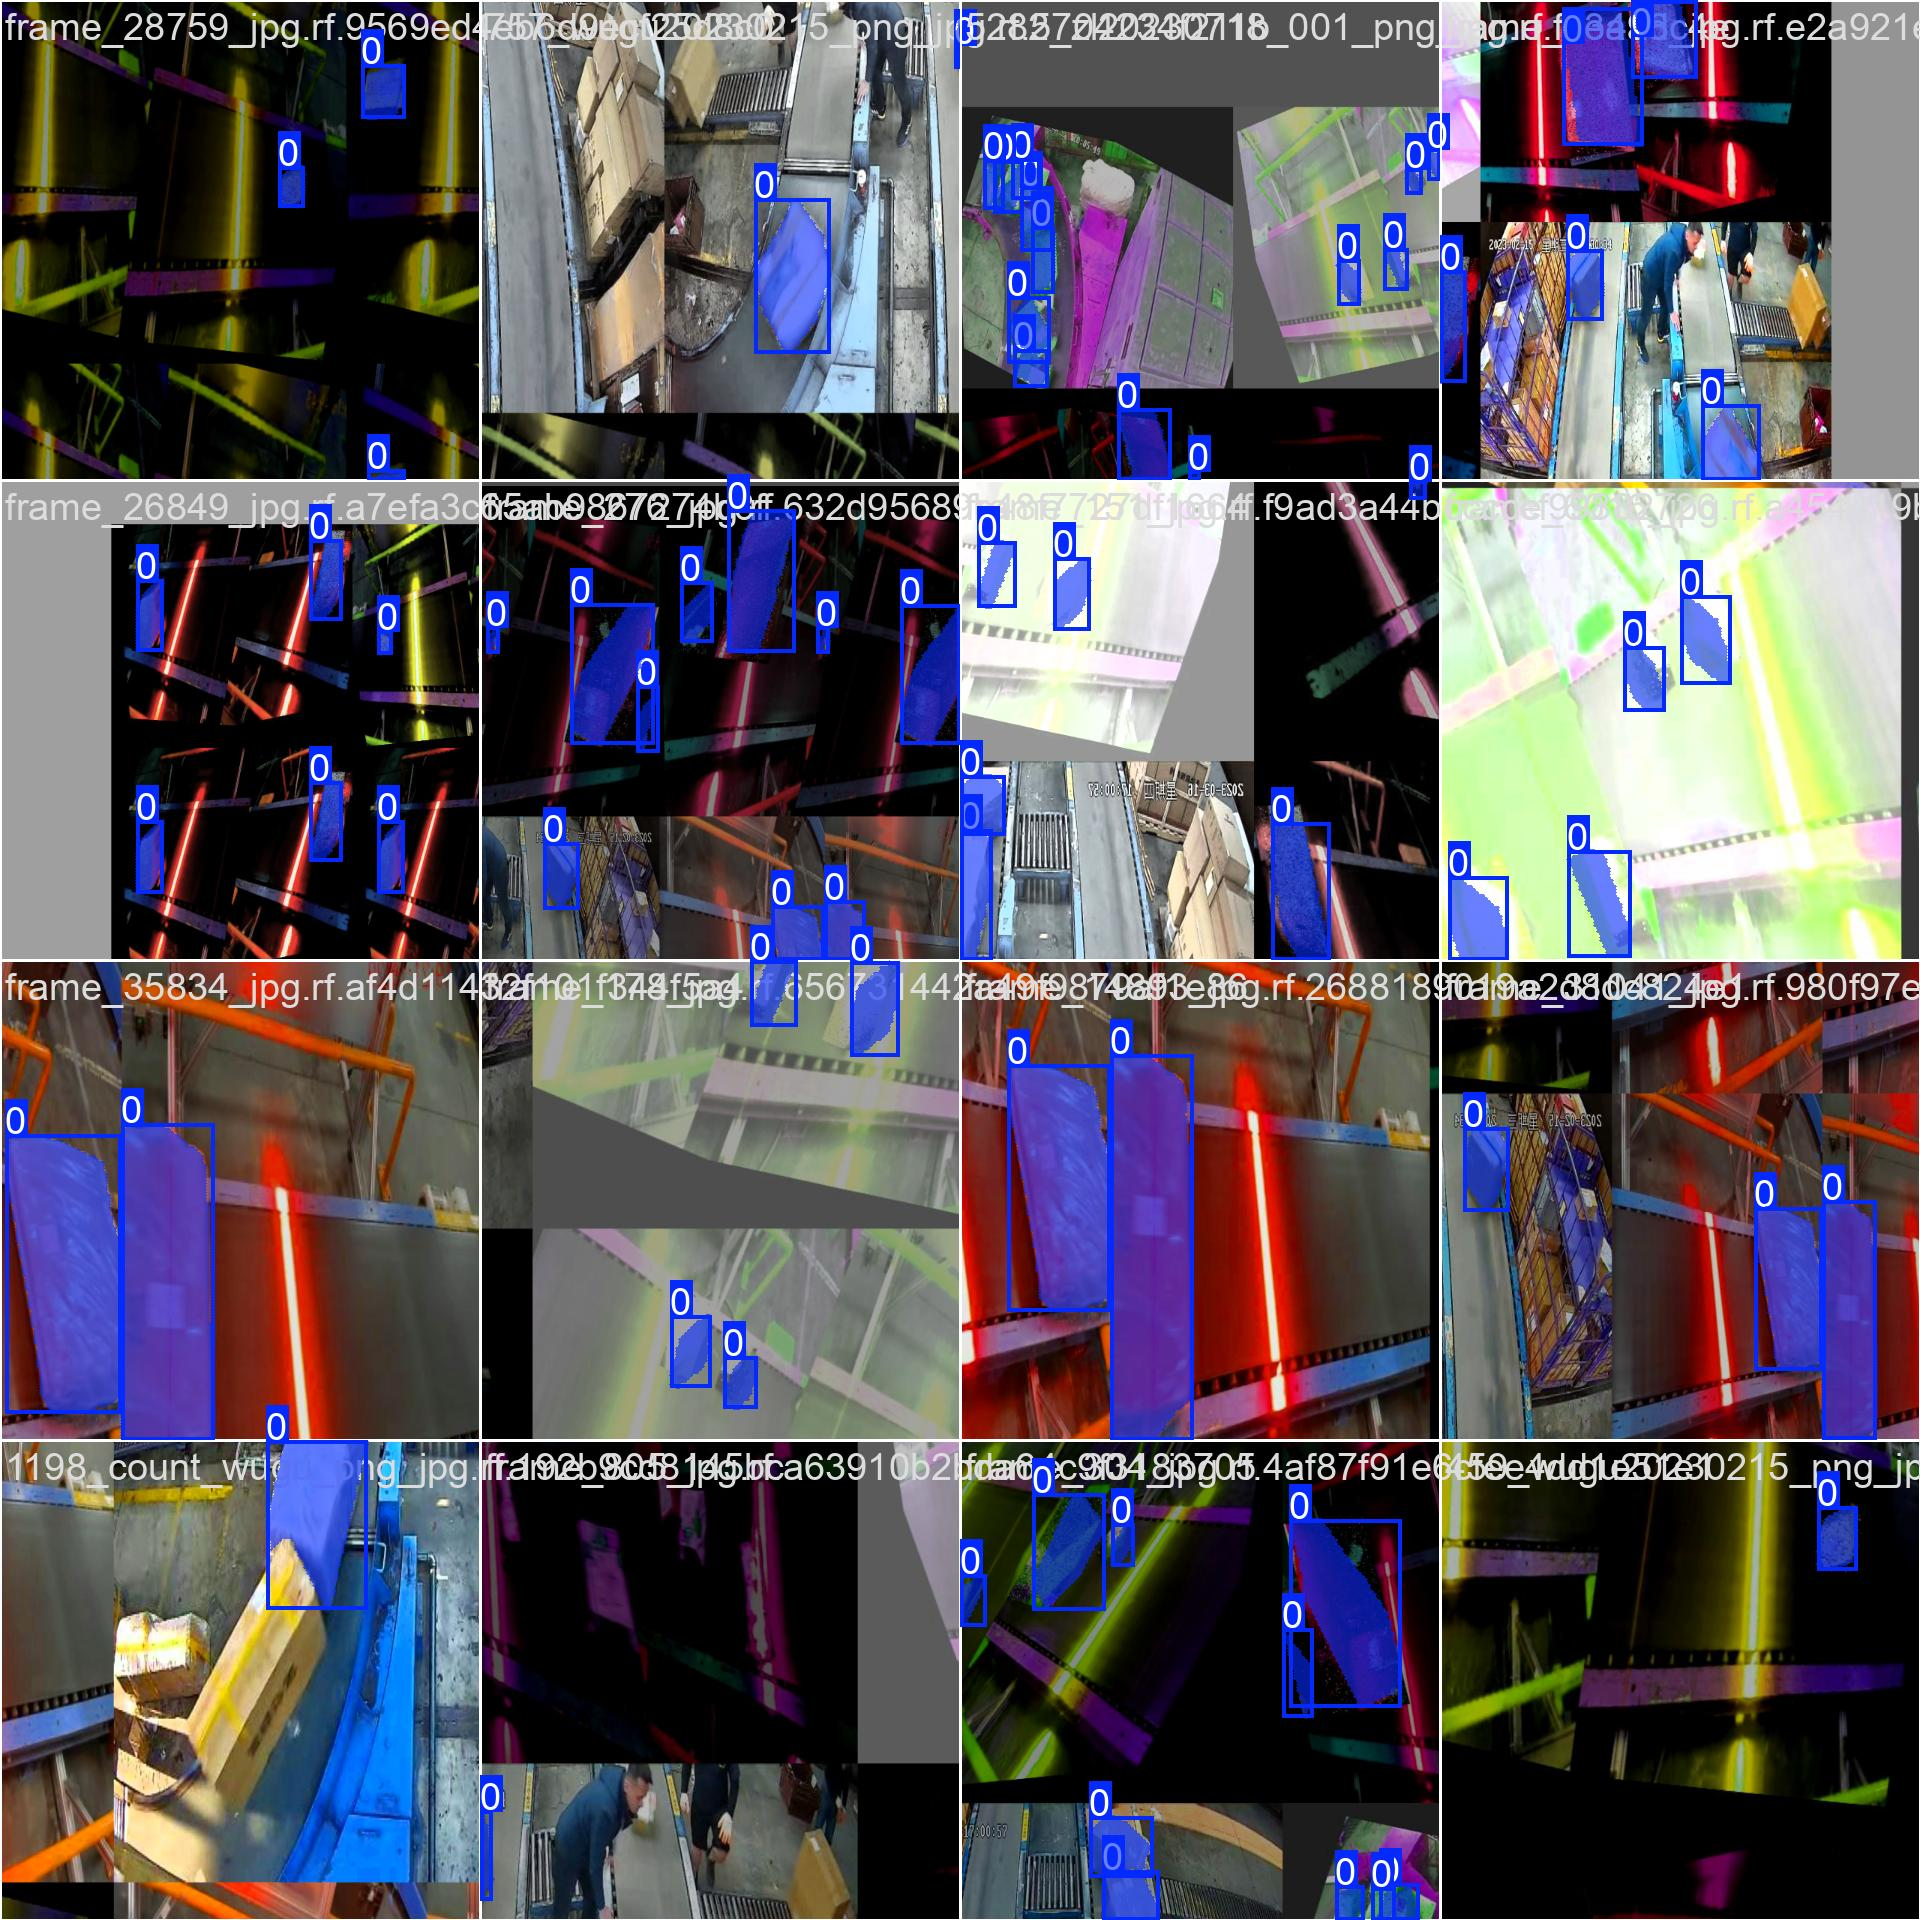
\includegraphics[width=0.52\textwidth]{train_batch.jpg}
\caption{Một lô ảnh huấn luyện do Ultralytics xuất ra, với mặt nạ nhãn tô màu chồng lên ảnh. Phép
tăng cường ghép ảnh (mosaic) dán bốn ảnh gốc vào một khung~\cite{bochkovskiy2020}. Có thể thấy
nhiều ảnh chứa cả chồng kiện hàng xếp sát nhau --- trường hợp khó nhất của bài toán.}
\label{fig:batch}
\end{figure}

\section{Phương pháp}

\subsection{Học chuyển giao thay vì huấn luyện từ đầu}

Với \ntrain{} ảnh thì huấn luyện từ đầu là không khả thi, nên em khởi tạo từ trọng số tiền huấn
luyện trên COCO~\cite{lin2014} và huấn luyện tiếp toàn bộ mạng. Lý do cách làm này hiệu quả đã được
Yosinski và cộng sự phân tích~\cite{yosinski2014}: các tầng đầu học những thứ chung cho mọi ảnh tự
nhiên nên tái dùng được gần như nguyên vẹn, càng về sau biểu diễn càng chuyên biệt cho bài toán gốc
và cần chỉnh lại.

Ở đây việc chuyển giao có một thuận lợi riêng: COCO có sẵn lớp \emph{box} và nhiều vật thể hình hộp
chữ nhật, nên biểu diễn về cạnh thẳng, góc vuông và mặt phẳng nghiêng đã có sẵn trong mạng. Phần
mô hình phải học thêm chủ yếu là tách hai kiện hàng cạnh nhau, việc mà dữ liệu COCO không dạy.

\subsection{Mô hình dự đoán cái gì}

So với bài phát hiện, hàm mất mát có thêm một thành phần. Ultralytics ghi riêng từng phần trong
nhật ký huấn luyện, và em dùng tổng của chúng khi vẽ hình:

\begin{itemize}
  \item \texttt{cls\_loss} --- mất mát phân lớp. Ở bài này chỉ có \nclasses{} lớp nên nó gần như
        chỉ còn nhiệm vụ phân biệt vật với nền.
  \item \texttt{box\_loss} --- mất mát định vị hộp. Đầu phân đoạn vẫn dự đoán hộp, vì mặt nạ được
        cắt theo hộp tương ứng trước khi xuất ra.
  \item \texttt{dfl\_loss} --- Distribution Focal Loss~\cite{li2020}: thay vì dự đoán mỗi cạnh hộp
        bằng một con số, mô hình dự đoán một phân phối rời rạc trên các vị trí khả dĩ rồi lấy kỳ
        vọng, nhờ đó biểu diễn được sự không chắc chắn ở những biên mờ.
  \item \texttt{seg\_loss} --- mất mát mặt nạ, thành phần riêng của bài này, so sánh mặt nạ dựng từ
        các nguyên mẫu với mặt nạ nhãn ở mức điểm ảnh.
\end{itemize}

Chỉ số đánh giá cũng đi theo hai nhánh. Ultralytics ký hiệu (B) cho các chỉ số tính trên hộp giới
hạn và (M) cho chỉ số tính trên mặt nạ. Cả hai đều dùng định nghĩa mAP quen thuộc~\cite{everingham2010},
chỉ khác ở chỗ độ chồng lấn được tính giữa hai mặt nạ thay vì giữa hai hộp. Báo cáo này lấy nhóm
(M) làm chỉ số chính, vì đó mới là thứ bài toán phân đoạn cần.

\subsection{Giao thức huấn luyện và phần mã cấu hình}

Vì phép so sánh ba cỡ mô hình là nội dung chính, giao thức huấn luyện phải giống nhau tuyệt đối
giữa ba lần chạy. Em gom toàn bộ giao thức vào một lớp dữ liệu duy nhất trong
\texttt{src/yolo/config.py}, dùng chung cho cả bài phát hiện và bài phân đoạn; chuyển bài toán chỉ
là đổi giá trị \texttt{task}, và hàm \texttt{weights()} tự chọn đúng họ điểm kiểm tra có hậu tố
\texttt{-seg}.

\begin{lstlisting}
SIZES = ("n", "s", "m")
VERSION = "yolo11"

DATASETS = {
    "detect": "african-wildlife.yaml",
    "segment": "package-seg.yaml",
}

def weights(size: str, task: str) -> str:
    suffix = "-seg" if task == "segment" else ""
    return f"{VERSION}{size}{suffix}.pt"

@dataclass(frozen=True)
class TrainConfig:
    """Everything that must be identical across the three model sizes."""
    task: str = "detect"      # "segment" cho bai tap nay
    epochs: int = 50
    imgsz: int = 416          # 640 khi chay tren GPU
    batch: int = 8            # 16 khi chay tren GPU
    seed: int = 42
    workers: int = 4
    device: str = "cpu"
    patience: int = 20
    optimizer: str = "auto"
    extra: dict = field(default_factory=dict)

    @property
    def data(self) -> str:
        return DATASETS[self.task]
\end{lstlisting}

\begin{table}[H]
\centering
\caption{Giao thức huấn luyện. Ba cỡ mô hình dùng đúng các giá trị này; điểm khác duy nhất giữa ba lần chạy là tệp trọng số khởi tạo. Toàn bộ tham số được khai báo một chỗ trong \texttt{src/yolo/config.py} nên không thể lệch nhau giữa các lần chạy.}
\label{tab:protocol}
\small
\begin{tabular}{l l}
\toprule
Tham số & Giá trị \\
\midrule
Phiên bản mô hình & YOLO11 (yolo11n-seg, yolo11s-seg, yolo11m-seg) \\
Trọng số khởi tạo & điểm kiểm tra tiền huấn luyện trên COCO của Ultralytics \\
Số epoch & 50 \\
Kích thước ảnh đầu vào & 640$\times$640 \\
Kích thước lô (batch) & 16 \\
Hạt giống ngẫu nhiên & 42 \\
Bộ tối ưu & tự động (\texttt{optimizer=auto}) theo Ultralytics \\
Tốc độ học & tăng tới 0{,}00192 sau 3 epoch khởi động, giảm dần còn $5{,}96\times 10^{-5}$ \\
Tăng cường dữ liệu & mặc định của Ultralytics; ghép ảnh (mosaic) tắt ở 10 epoch cuối \\
Kiên nhẫn dừng sớm & 20 epoch (không mô hình nào bị dừng sớm) \\
Phần cứng & GPU NVIDIA A100-SXM4-40GB trên Google Colab \\
Phiên bản thư viện & Ultralytics 8.4.192, Python 3.13.16, torch 2.11.0+cu130 \\
\bottomrule
\end{tabular}
\end{table}


Vòng lặp huấn luyện trong \texttt{src/yolo/train.py} chỉ làm ba việc: nạp điểm kiểm tra tương ứng
với cỡ mô hình, gọi \texttt{model.train()} với bộ tham số sinh từ cấu hình trên, rồi chấm điểm
trên phần \emph{test} bằng \texttt{model.val(split="test")}. Em không cài lại phần nào của YOLO. Tệp
kết quả ghi kèm toàn bộ tham số giao thức bên cạnh các chỉ số, nên bảng kết quả luôn mang theo điều
kiện đã sinh ra nó.

Ba mô hình được huấn luyện lần lượt trên GPU Tesla T4 của Google Colab, tổng cộng \totalminutes{}
phút --- gấp hơn hai lần bài phát hiện, đúng như dự đoán từ số ảnh huấn luyện và từ việc có thêm
nhánh mặt nạ.

\section{Kết quả}

\begin{table}[H]
\centering
\caption{Kết quả trên tập giữ lại (test). Dòng cuối bảng là độ lệch chuẩn của mAP50-95 trong mười epoch cuối, đo trên tập val. Mức dao động lớn nhất (0{,}0100) lớn hơn khoảng cách giữa ba mô hình trên tập val (0{,}0097), nên thứ tự ba dòng trên không nên đọc như một bảng xếp hạng. Ký hiệu (M) chỉ chỉ số tính trên mặt nạ.}
\label{tab:results}
\small
\begin{tabular}{l r r r r r r}
\toprule
Mô hình & Tham số (M) & Thời gian (phút) & Precision & Recall & mAP50 & mAP50-95 \\
\midrule
yolo11n-seg & 2{,}9 & 12{,}7 & 0{,}926 & 0{,}962 & 0{,}9673 & 0{,}8453 \\
yolo11s-seg & 10{,}1 & 12{,}9 & 0{,}903 & 0{,}945 & 0{,}9654 & 0{,}8507 \\
yolo11m-seg & 22{,}4 & 15{,}6 & 0{,}901 & 0{,}957 & 0{,}9588 & \textbf{0{,}8568} \\
\midrule
\multicolumn{7}{l}{\small Dao động mAP50-95 trên val, 10 epoch cuối: yolo11n-seg 0{,}0090; yolo11s-seg 0{,}0038; yolo11m-seg 0{,}0100} \\
\bottomrule
\end{tabular}
\end{table}


Cả ba mô hình đều đạt mAP50 của mặt nạ trên 0,95: với ngưỡng chồng lấn dễ dãi 0,5 thì gần như mọi
kiện hàng đều được tìm thấy và khoanh vùng hợp lý. Chỉ số khắt khe mAP50-95, lấy trung bình qua
mười ngưỡng chồng lấn từ 0,5 đến 0,95, giảm xuống khoảng 0,85 --- phần sai còn lại nằm ở độ sát của
đường viền chứ không phải ở việc bỏ sót vật.

\begin{figure}[H]
\centering
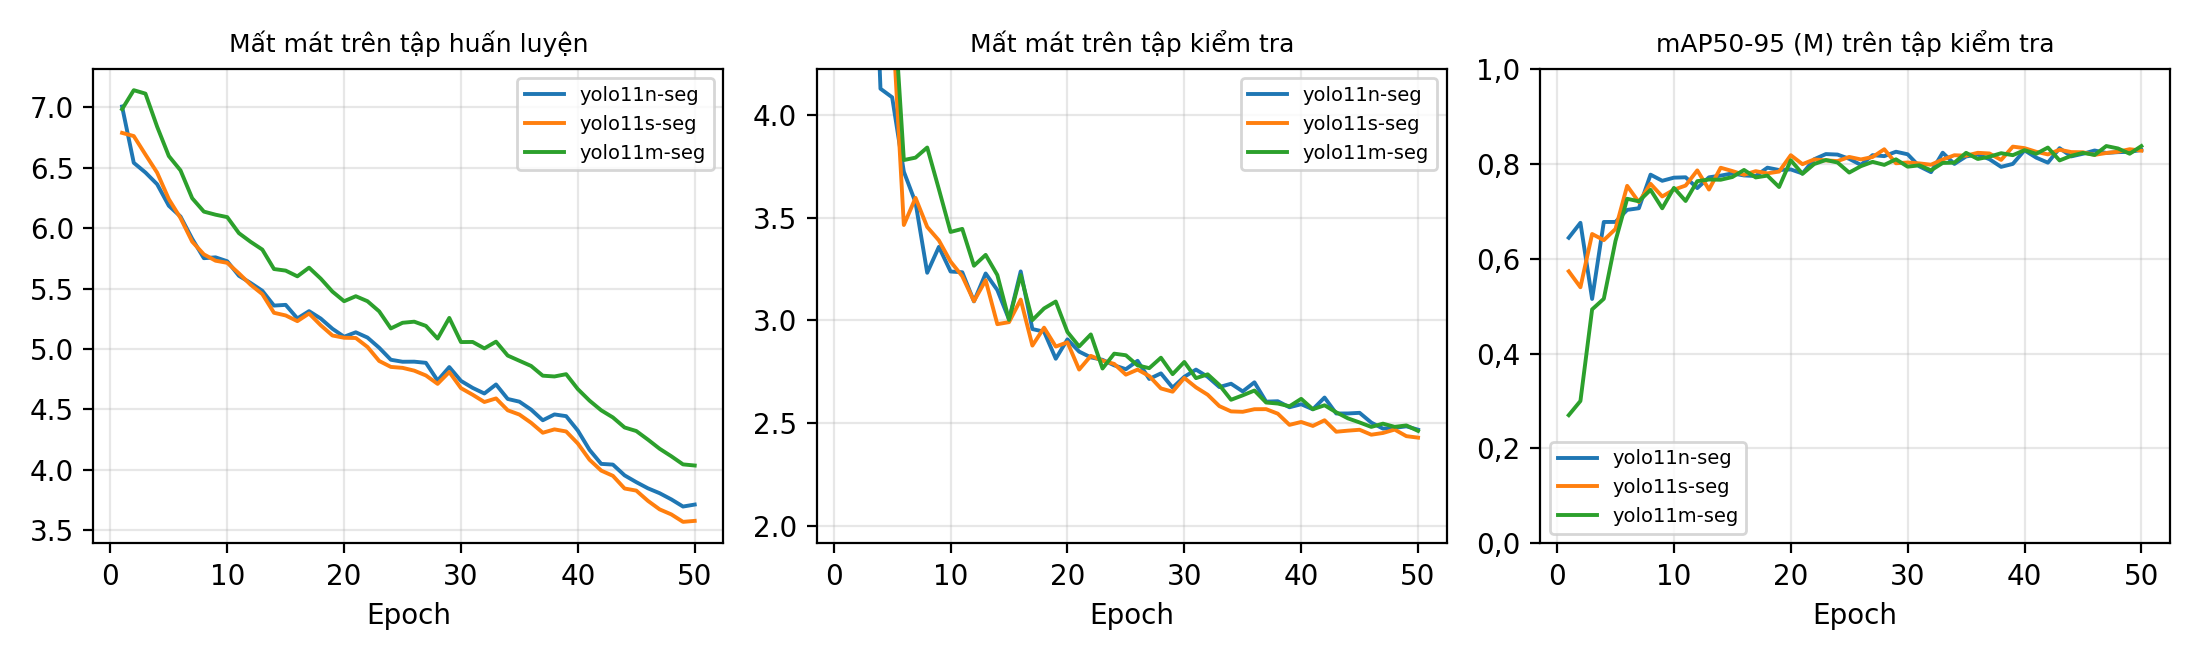
\includegraphics[width=\textwidth]{curves.png}
\caption{Mất mát và mAP mặt nạ theo từng epoch của ba mô hình, vẽ chung trục để so sánh được. Trục
đứng của ô giữa được cắt ngay trên mức mất mát từ epoch 8 trở đi, vì những epoch đầu vọt rất cao và
sẽ làm phẳng toàn bộ phần còn lại.}
\label{fig:curves}
\end{figure}

Hình~\ref{fig:curves} và Hình~\ref{fig:ultralytics} là bằng chứng huấn luyện mà đề bài yêu cầu;
Bảng~\ref{tab:log} bổ sung phần nhật ký thô do chính Ultralytics ghi ra sau mỗi epoch, để đối
chiếu được với các hình. Ba điều đọc được từ các đường cong:

\begin{itemize}
  \item Mất mát trên cả hai tập đều giảm đều và không tách nhau ở cuối, nên không có dấu hiệu quá
        khớp.
  \item Mô hình lớn nhất có mất mát huấn luyện \emph{cao hơn} hai mô hình kia trong suốt quá
        trình. Điều này thoạt nghe vô lý vì mô hình nhiều tham số lẽ ra phải khớp dữ liệu dễ hơn,
        nhưng với \epochs{} epoch thì nó đơn giản là chưa đi hết được quãng đường của mình.
  \item Đường mAP của ba mô hình chồng lên nhau gần như hoàn toàn từ epoch 10 trở đi. Đây là quan
        sát dẫn tới phần phân tích bên dưới.
\end{itemize}

\begin{table}[H]
\centering
\caption{Trích nhật ký huấn luyện của yolo11n-seg, chép trực tiếp từ \texttt{runs/segment/yolo11n/results.csv} --- tệp do Ultralytics ghi sau mỗi epoch trong lúc chạy. Cột thời gian là giây tính từ lúc bắt đầu.}
\label{tab:log}
\small
\begin{tabular}{r r r r r r}
\toprule
Epoch & Thời gian (s) & Mất mát HL & Mất mát KT & mAP50 (M) & mAP50-95 (M) \\
\midrule
1 & 20{,}6 & 7{,}008 & 4{,}368 & 0{,}8299 & 0{,}6438 \\
2 & 35{,}6 & 6{,}541 & 4{,}623 & 0{,}8514 & 0{,}6752 \\
3 & 50{,}4 & 6{,}461 & 5{,}607 & 0{,}7175 & 0{,}5149 \\
\multicolumn{6}{c}{\dots} \\
49 & 723{,}7 & 3{,}694 & 2{,}484 & 0{,}9331 & 0{,}8247 \\
50 & 738{,}0 & 3{,}711 & 2{,}468 & 0{,}9328 & 0{,}8287 \\
\bottomrule
\end{tabular}
\end{table}


\begin{figure}[H]
\centering
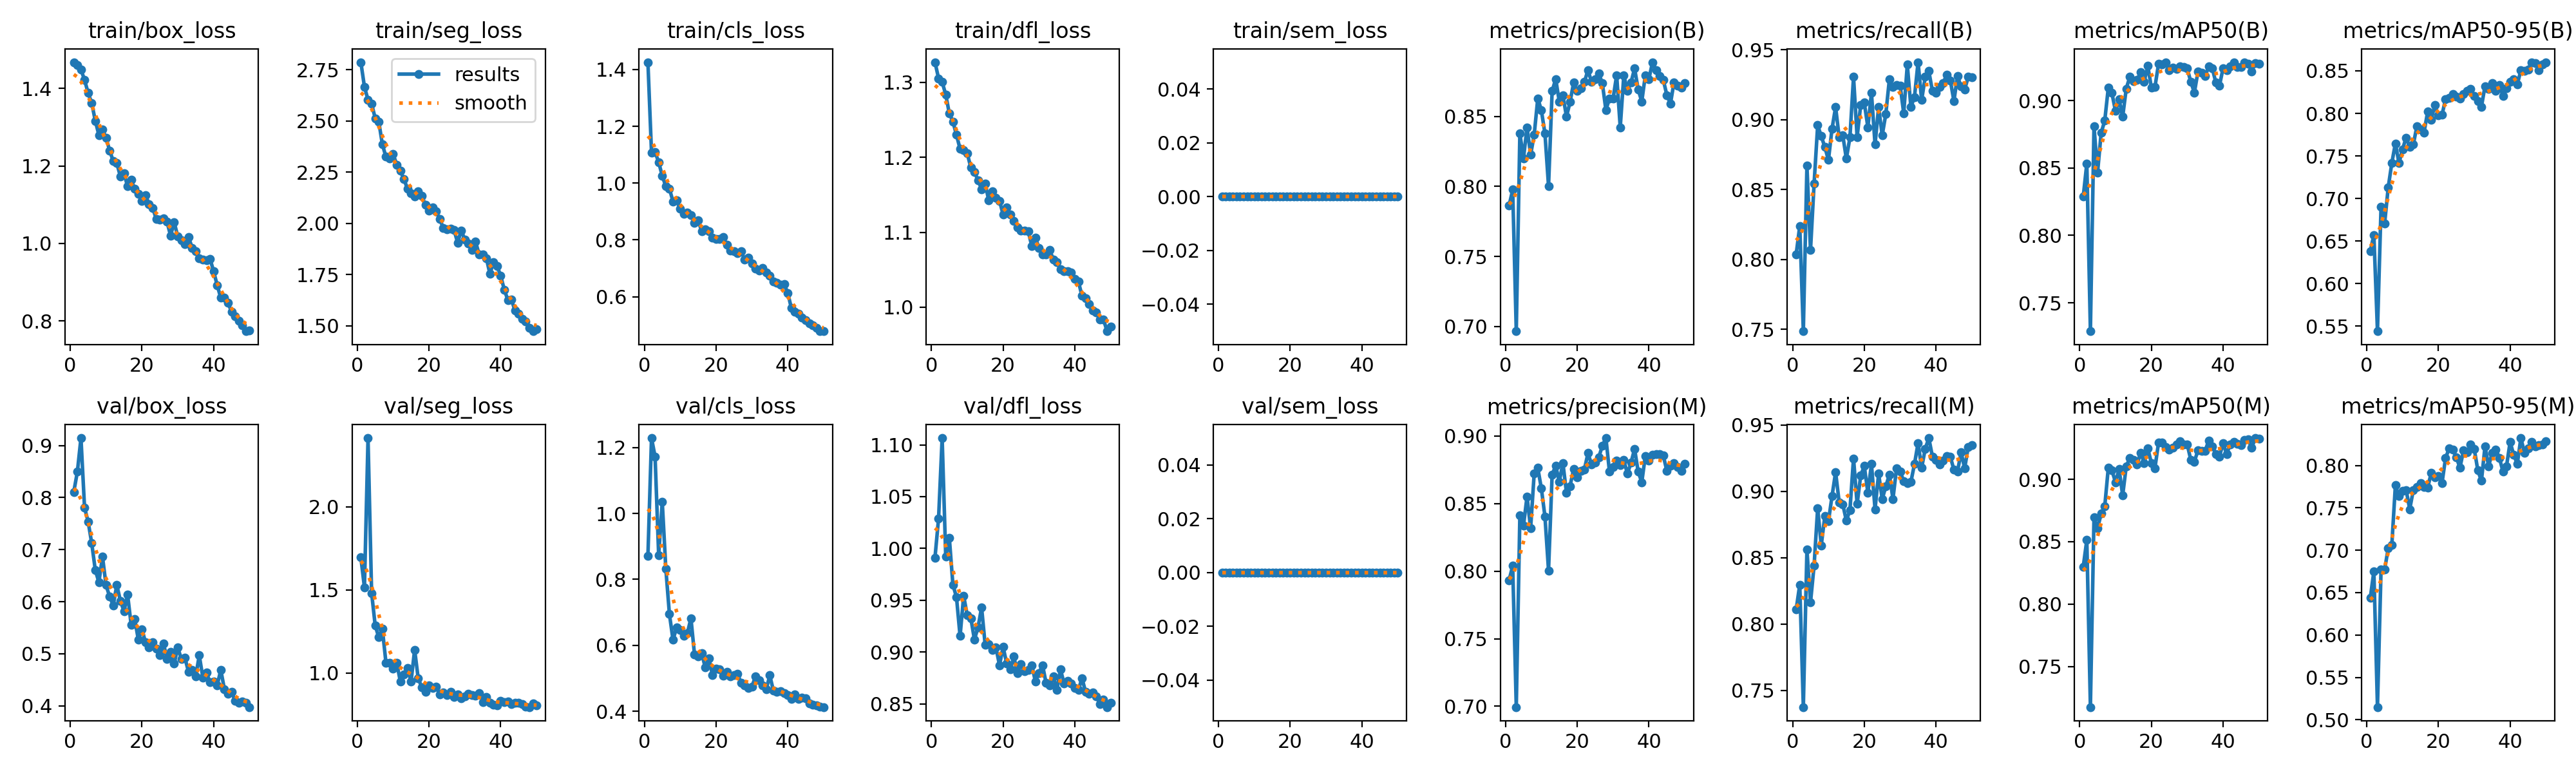
\includegraphics[width=0.68\textwidth]{ultralytics_n.png}
\caption{Toàn bộ nhật ký huấn luyện của yolo11n-seg do Ultralytics tự xuất ra
(\texttt{runs/segment/yolo11n/results.png}): bốn thành phần mất mát trên tập huấn luyện và tập kiểm
tra, cùng precision, recall, mAP50 và mAP50-95 cho cả hộp (B) và mặt nạ (M).}
\label{fig:ultralytics}
\end{figure}

\begin{figure}[H]
\centering
\begin{minipage}{0.48\textwidth}
  \centering
  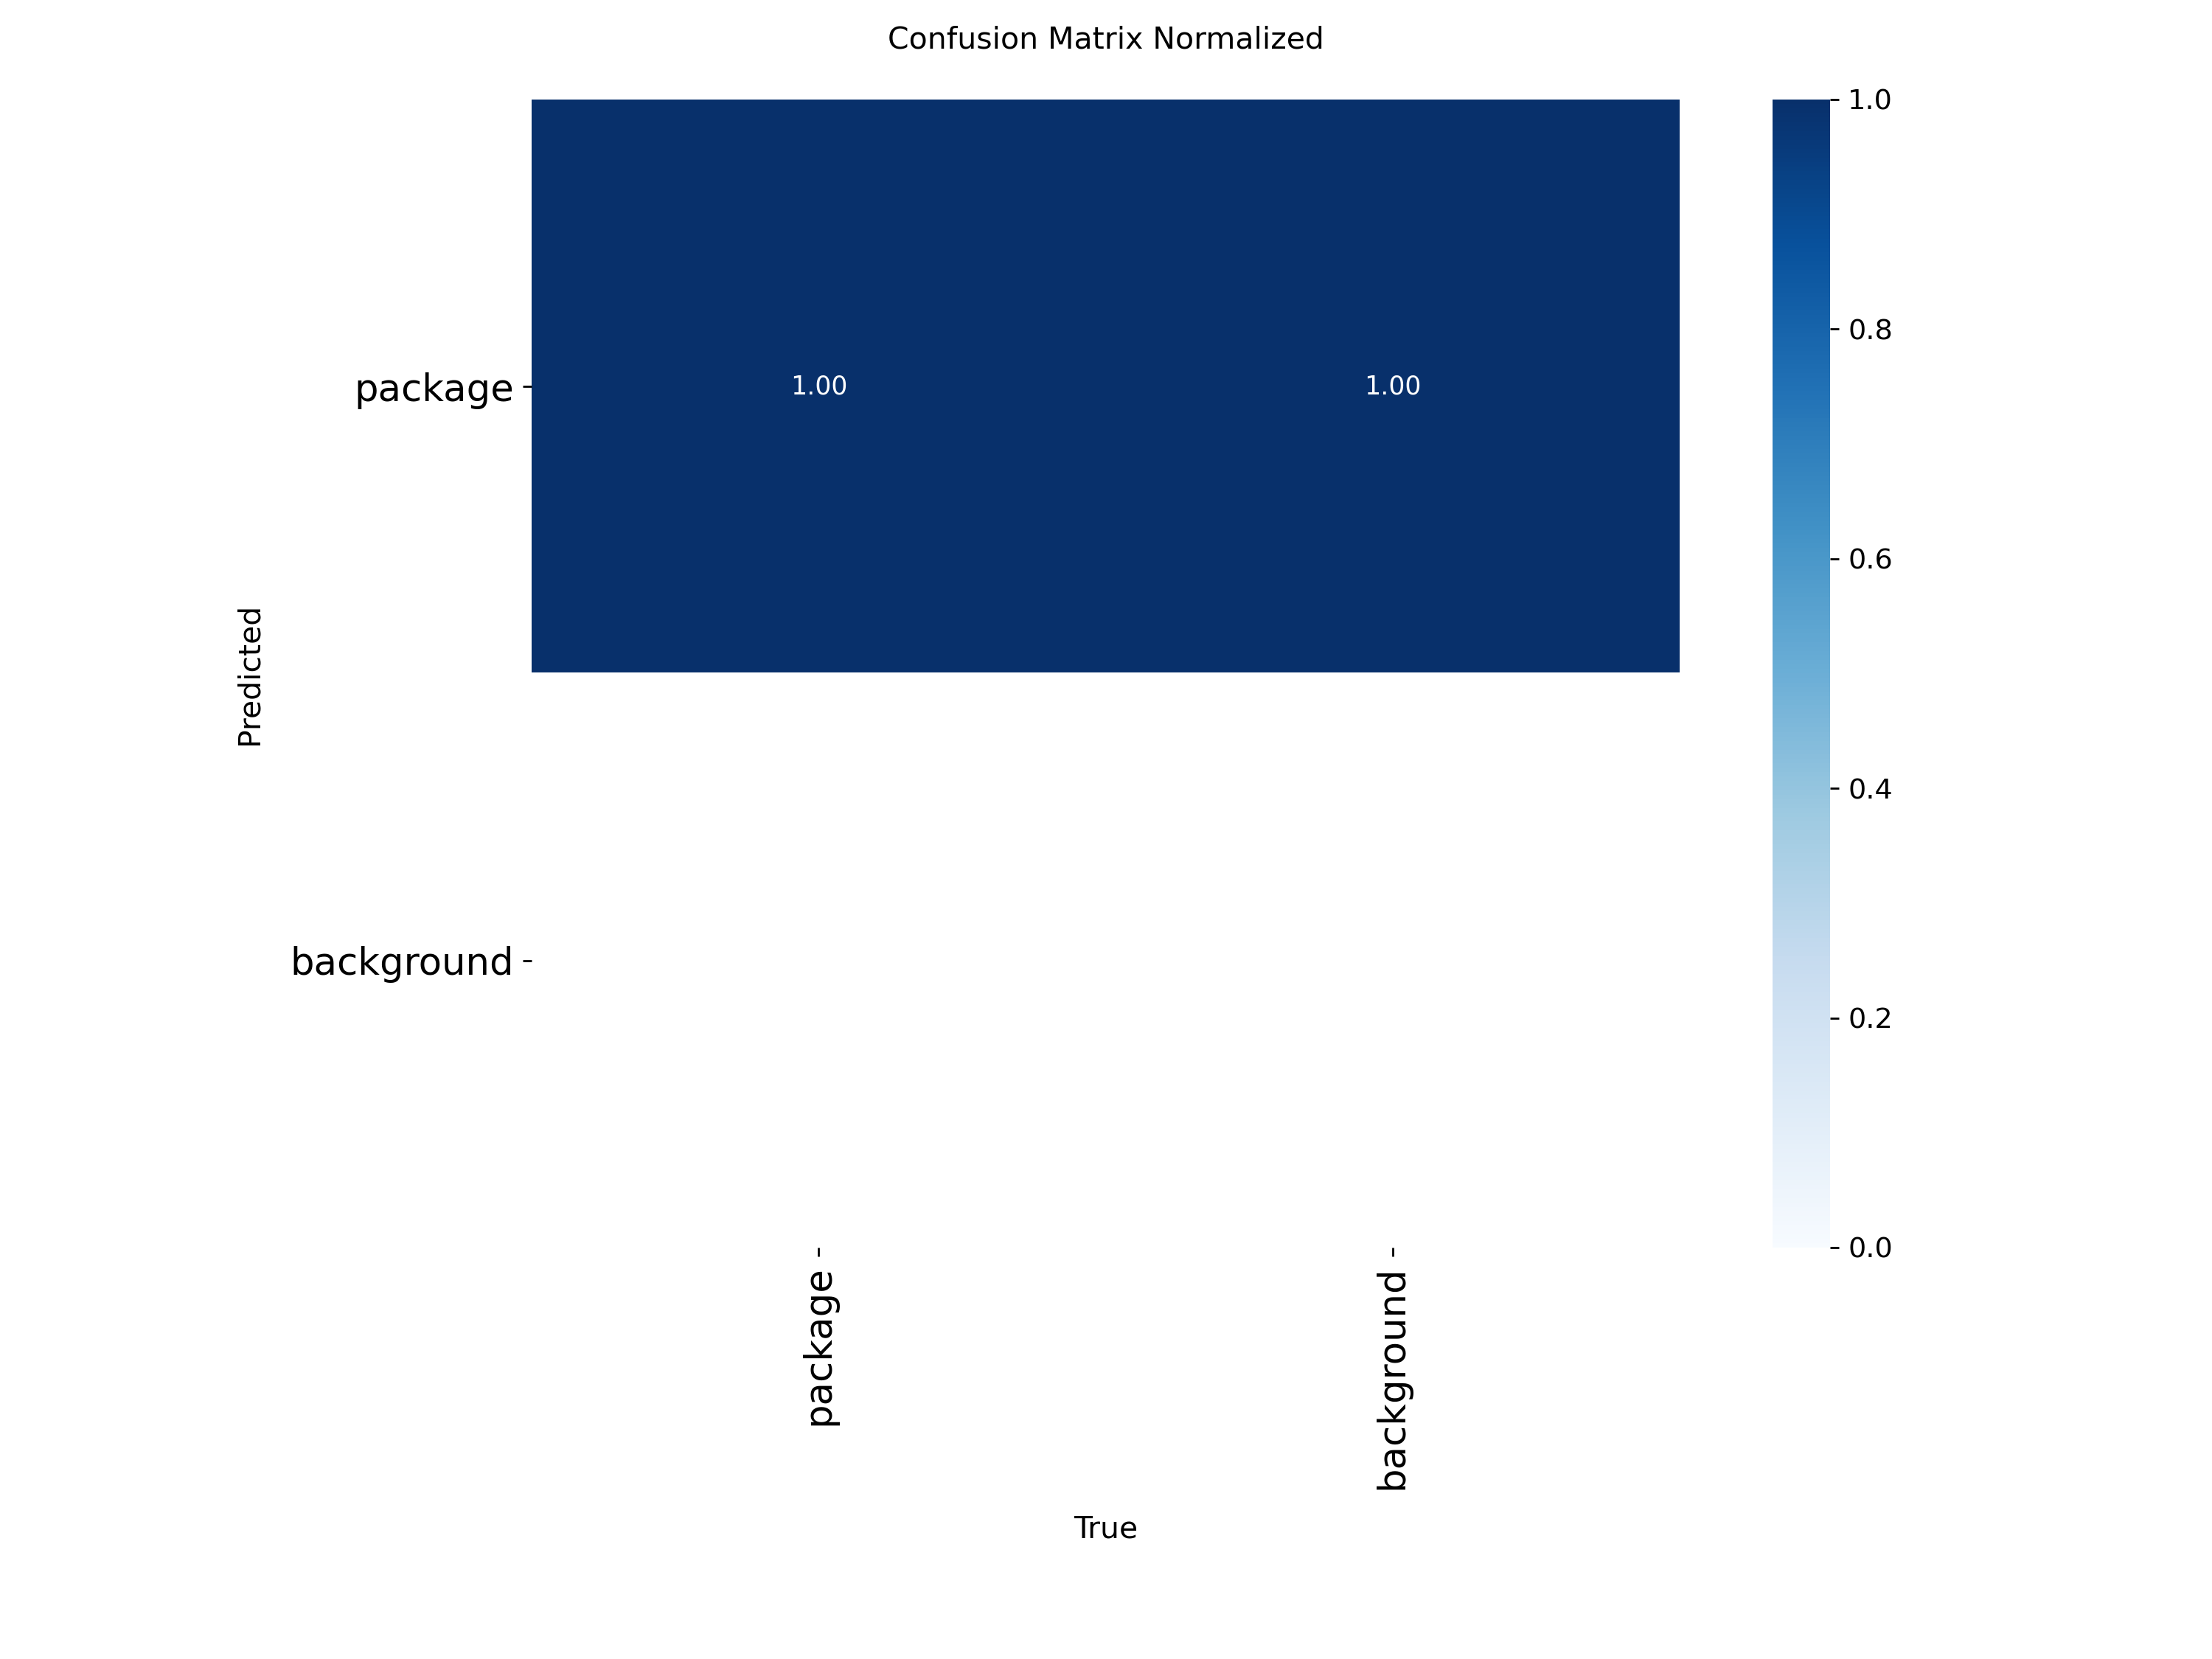
\includegraphics[width=\textwidth]{confusion.png}
\end{minipage}\hfill
\begin{minipage}{0.48\textwidth}
  \centering
  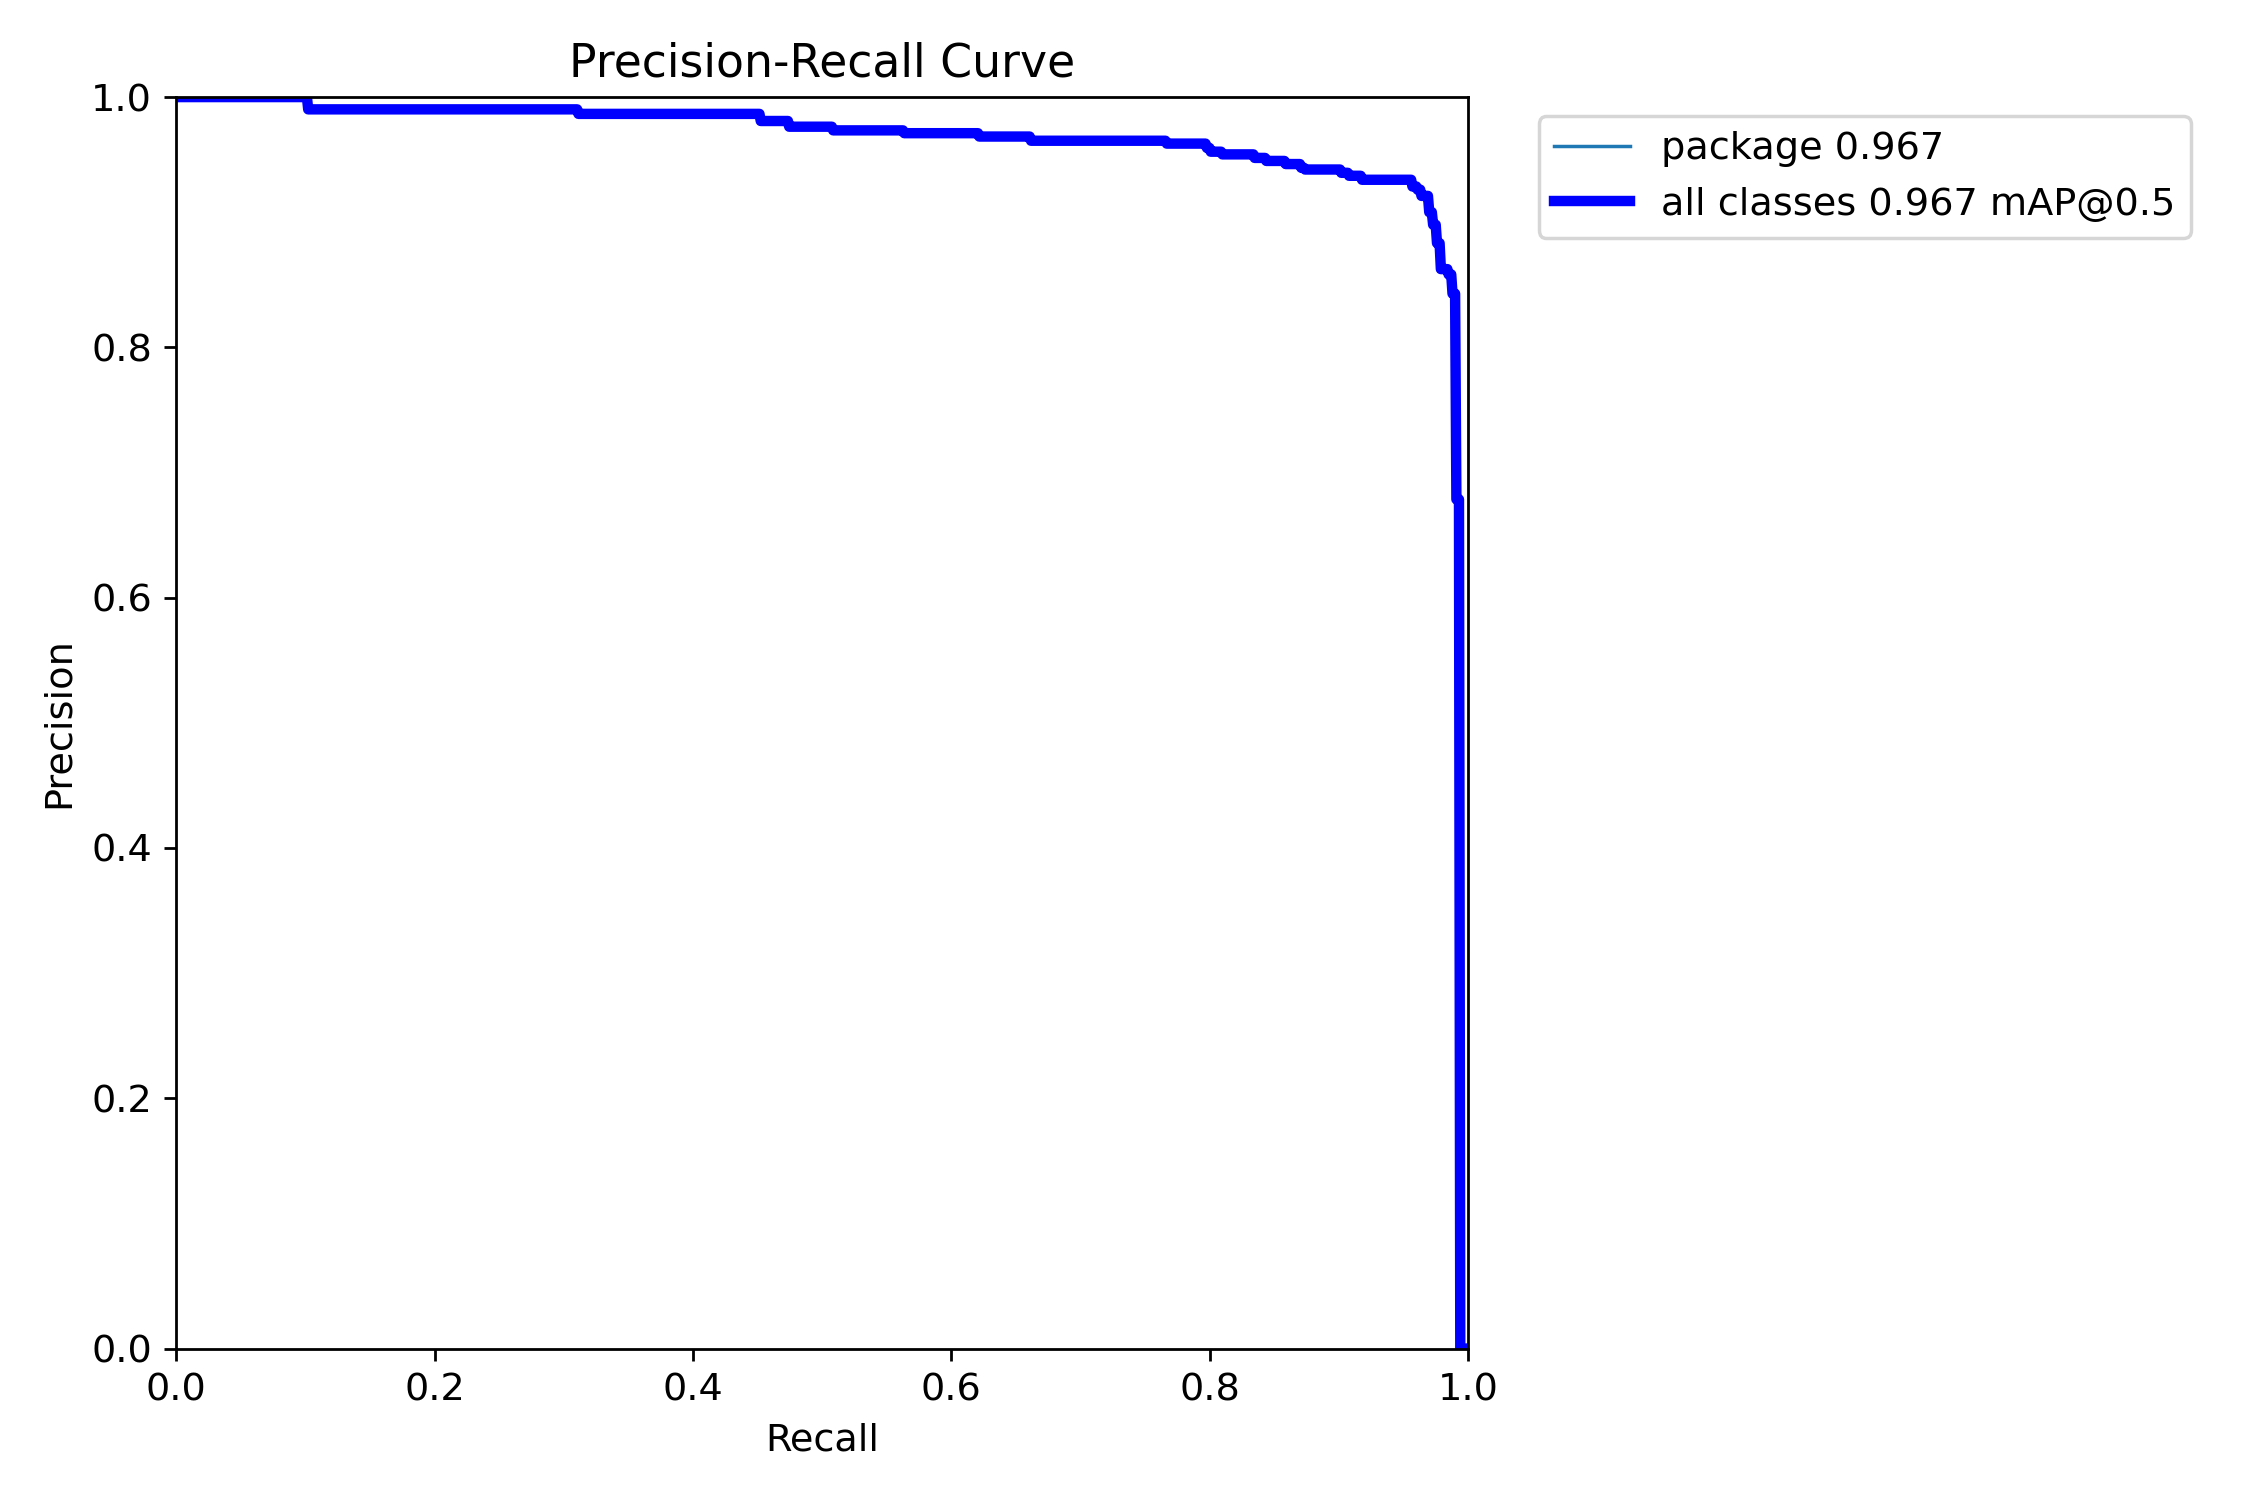
\includegraphics[width=\textwidth]{pr_curve.png}
\end{minipage}
\caption{Trái: ma trận nhầm lẫn chuẩn hoá của yolo11n-seg trên phần test. Phải: đường
precision--recall của mặt nạ. Vì chỉ có \nclasses{} lớp nên ma trận chỉ còn hai ô có nghĩa: bỏ sót
kiện hàng, và báo nhầm một vùng nền thành kiện hàng.}
\label{fig:confusion}
\end{figure}

Ma trận nhầm lẫn ở đây ít thông tin hơn hẳn bài phát hiện, đúng như em dự liệu khi chọn bộ dữ liệu
một lớp: không có chuyện nhầm lớp này với lớp kia, chỉ còn nhầm vật với nền. Bù lại, đường
precision--recall vẫn cho thấy được điều đáng quan tâm --- precision giữ ở mức cao cho tới khi
recall vượt khoảng 0,9, nghĩa là những kiện hàng cuối cùng mà mô hình cố tìm ra mới là nguồn của
phần lớn cảnh báo sai.

\begin{figure}[H]
\centering
\begin{minipage}{0.48\textwidth}
  \centering
  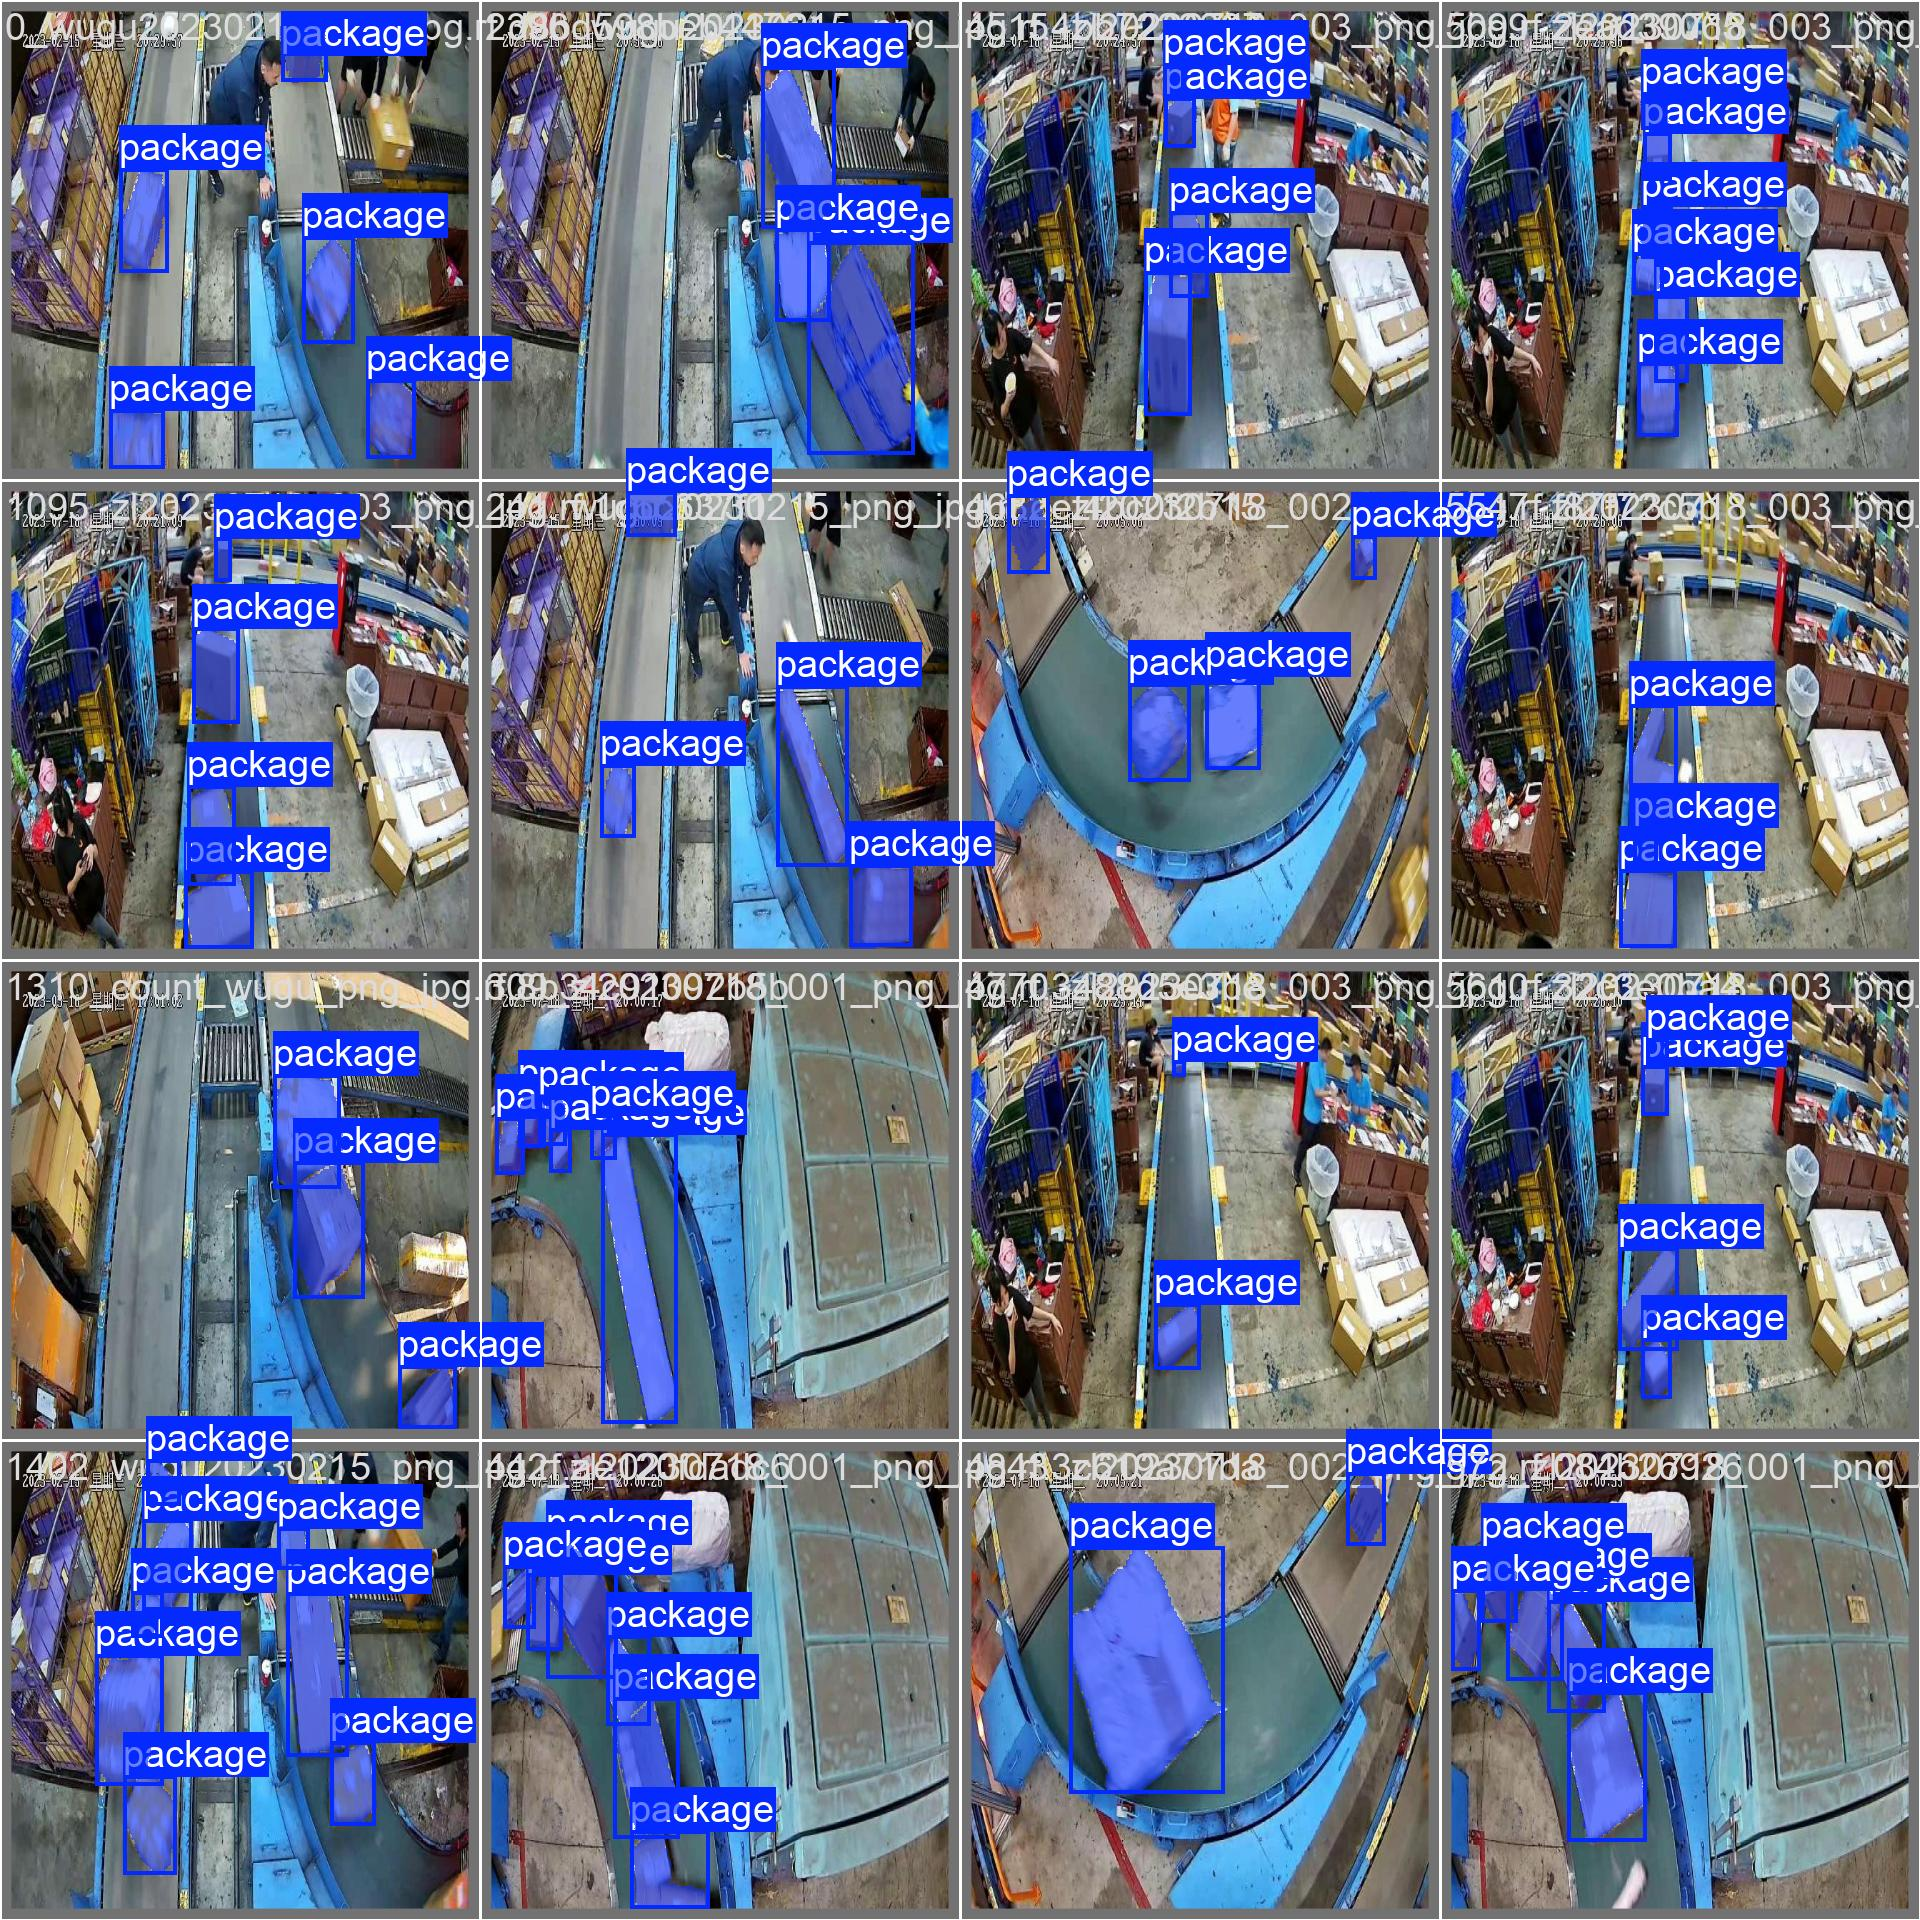
\includegraphics[width=\textwidth]{ground_truth.jpg}\\ {\small Mặt nạ nhãn}
\end{minipage}\hfill
\begin{minipage}{0.48\textwidth}
  \centering
  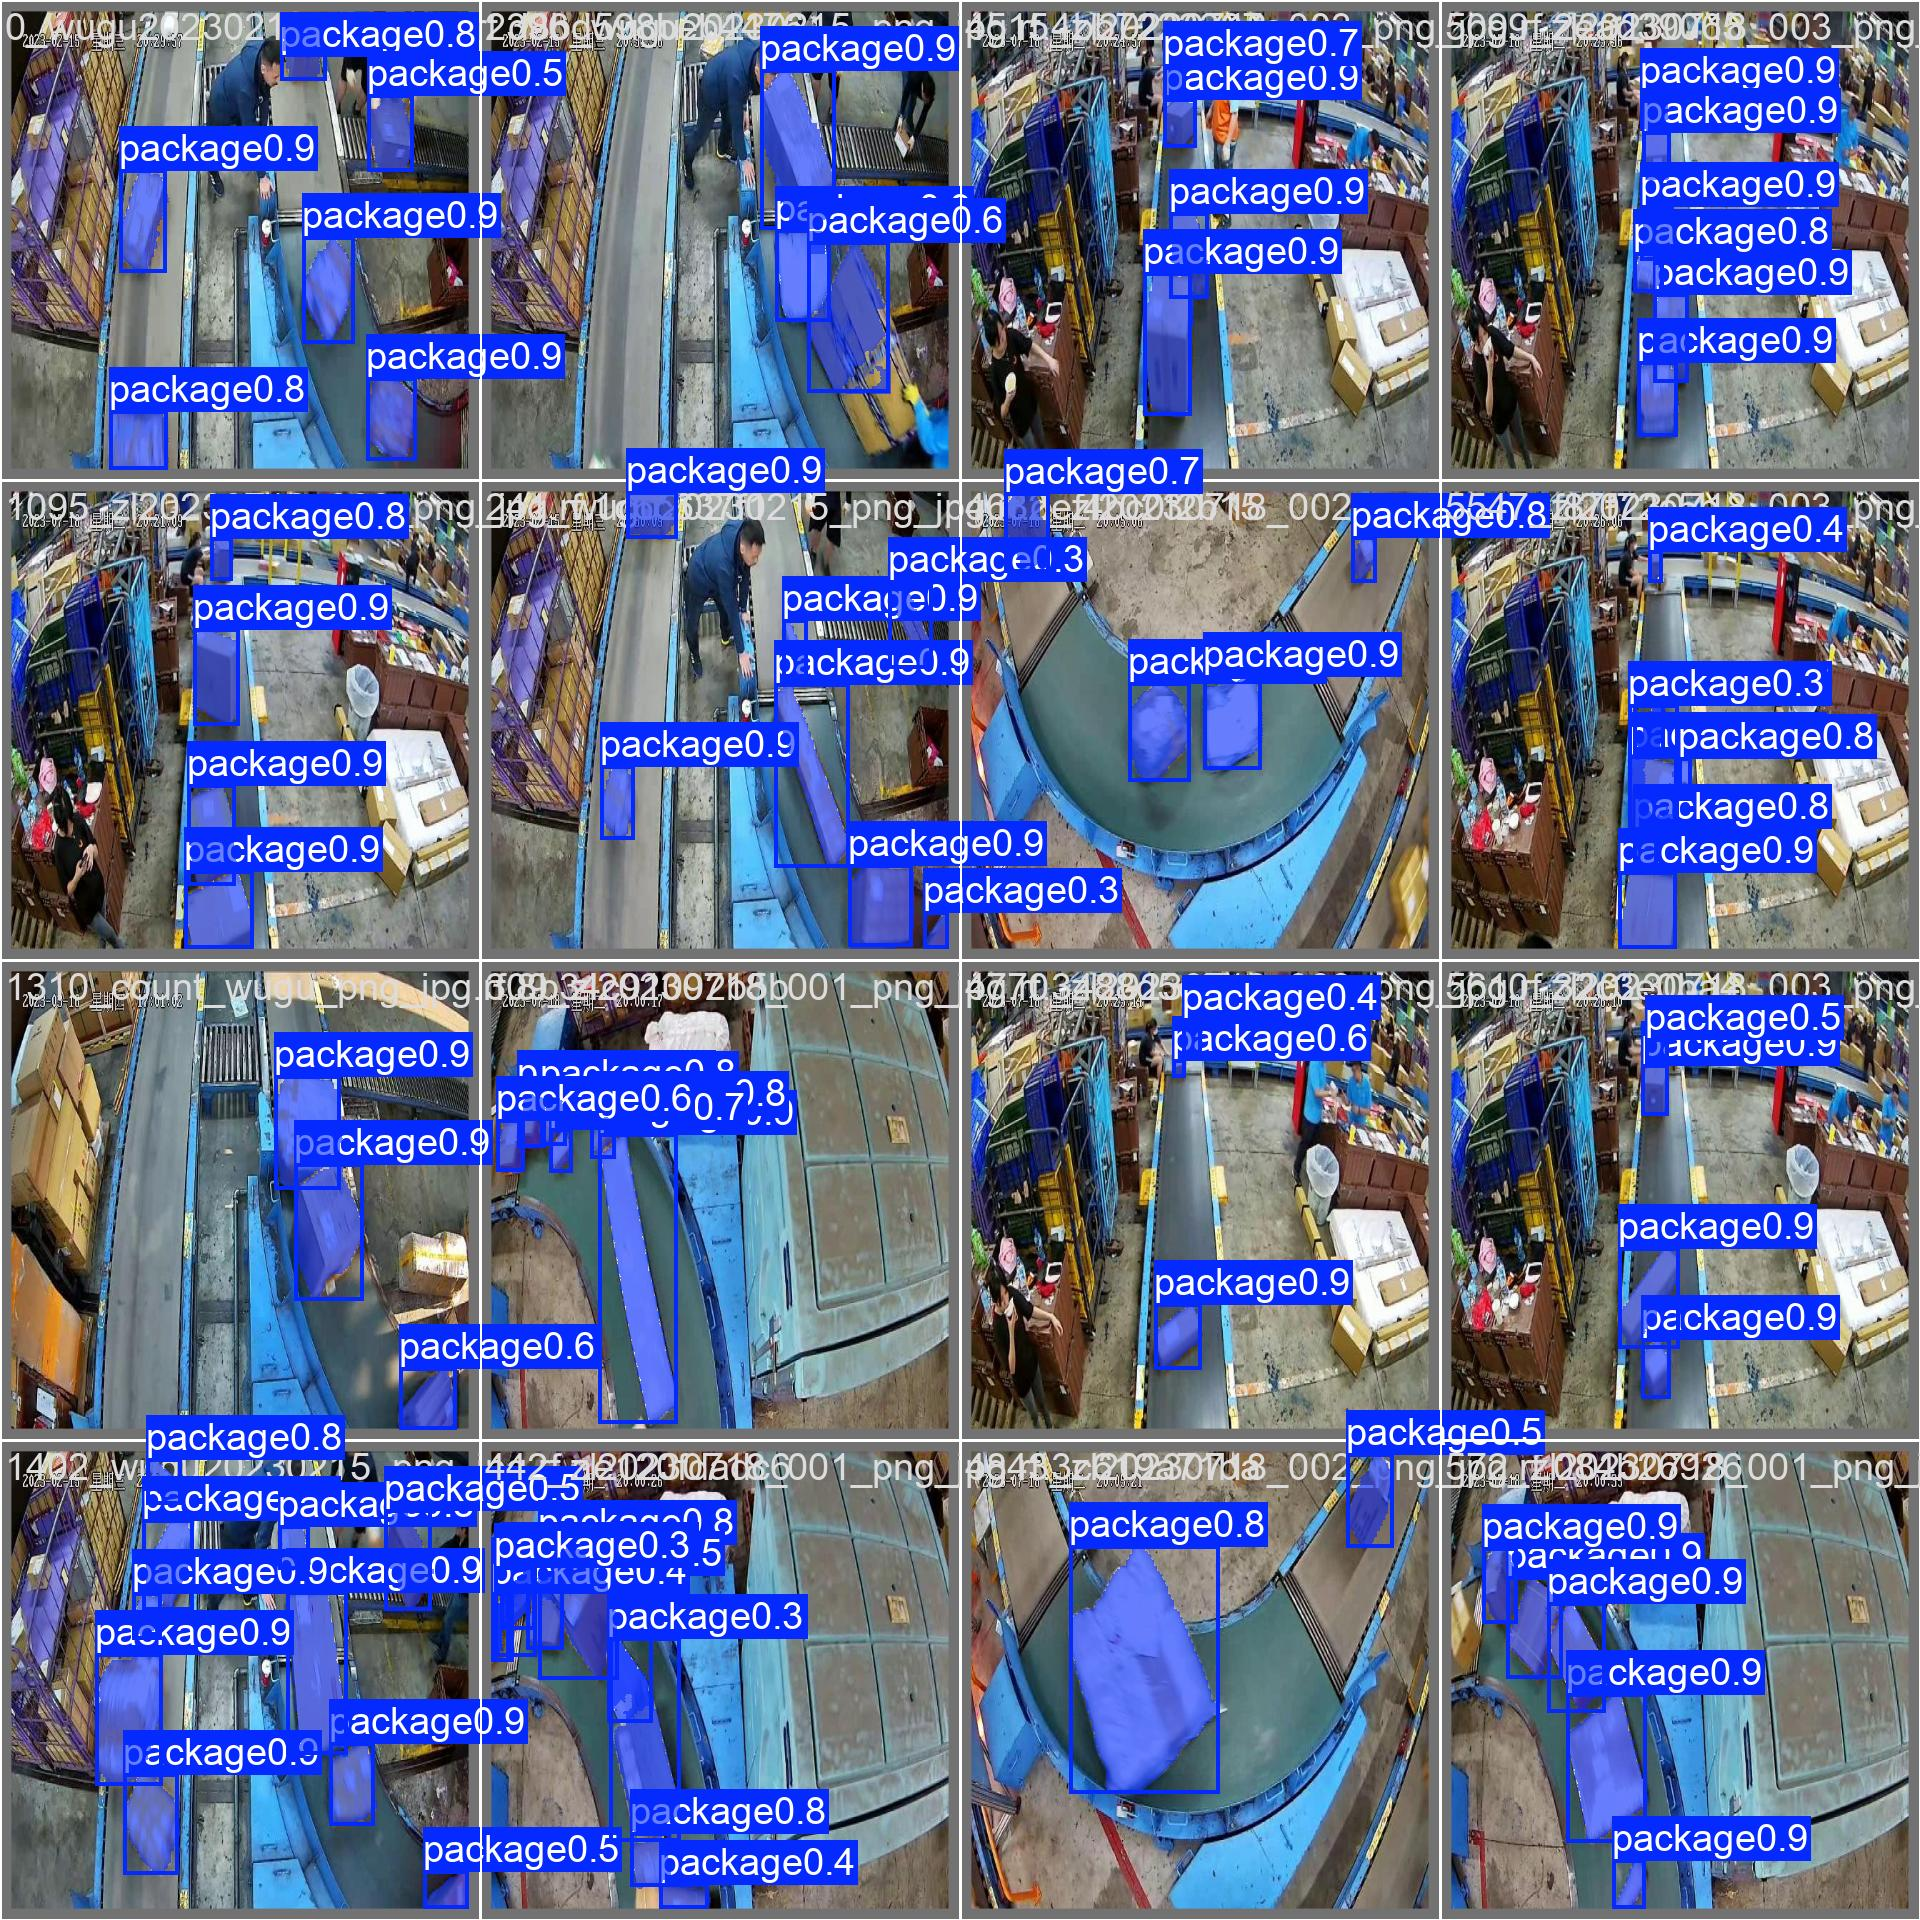
\includegraphics[width=\textwidth]{predictions.jpg}\\ {\small Dự đoán của yolo11n-seg}
\end{minipage}
\caption{Một lô ảnh trong phần test: mặt nạ do người gán (trái) và mặt nạ mô hình dự đoán (phải),
kèm điểm tin cậy. Các trường hợp còn sai thường là hai kiện hàng cùng màu xếp sát nhau bị gộp thành
một vùng, hoặc viền bị cắt thiếu ở chỗ bị che khuất.}
\label{fig:predictions}
\end{figure}

\subsection{Vẽ mặt nạ khó hơn vẽ hộp bao nhiêu}

Vì mô hình phân đoạn chấm điểm cả hộp lẫn mặt nạ trên cùng một lần chạy, có thể so sánh trực tiếp
hai nhánh chỉ số. Trên phần test, mAP50-95 của hộp là \nmapbox{} (yolo11n-seg), \smapbox{}
(yolo11s-seg) và \mmapbox{} (yolo11m-seg), đều cao hơn chỉ số tương ứng của mặt nạ; trung bình
khoảng cách là \maskboxgap{} điểm.

Khoảng cách này là cái giá của việc phải bám theo đường viền thật. Một hộp chữ nhật chỉ cần bốn số
đúng, còn mặt nạ phải đúng ở từng điểm ảnh dọc theo chu vi --- mà chu vi lại chính là chỗ nhãn của
con người cũng không thật sự chính xác: viền thùng carton bị mờ, bị che một phần, hoặc nằm sát một
thùng khác. Đáng chú ý là khoảng cách chỉ khoảng ba điểm rưỡi chứ không lớn hơn, cho thấy sơ đồ mặt
nạ nguyên mẫu dựng được đường viền khá sát dù chỉ dùng 32 nguyên mẫu dùng chung cho toàn ảnh.

\section{Phân tích: ba cỡ mô hình có thật sự khác nhau không?}

\begin{table}[H]
\centering
\caption{Cùng một chỉ số, đo trên hai tập dữ liệu khác nhau. Hai cột thống nhất ở mô hình đứng đầu nhưng đổi chỗ hai mô hình còn lại, trong khi khoảng cách giữa chúng chỉ xấp xỉ mức dao động của chính mỗi mô hình giữa các epoch.}
\label{tab:ordering}
\small
\begin{tabular}{l r r}
\toprule
Mô hình & mAP50-95 trên val & mAP50-95 trên test \\
\midrule
yolo11n-seg & 0{,}8287 & 0{,}8453 \\
yolo11s-seg & 0{,}8271 & 0{,}8507 \\
yolo11m-seg & 0{,}8369 & 0{,}8568 \\
\midrule
Khoảng cách lớn nhất--nhỏ nhất & 0{,}0097 & 0{,}0115 \\
\bottomrule
\end{tabular}
\end{table}


Trên phần test, mAP50-95 của mặt nạ tăng đều theo cỡ mô hình: \nmaptest{}, \smaptest{},
\mmaptest{}. Nhìn riêng cột đó thì kết luận có vẻ rõ ràng --- mô hình lớn hơn cho mặt nạ sát viền
hơn. Nhưng có ba điều khiến em không kết luận như vậy.

\textbf{Thứ nhất, hai chỉ số cho hai thứ tự ngược nhau.} Ở mAP50, thứ tự là \nmapfifty{} cho
yolo11n-seg, \smapfifty{} cho yolo11s-seg và \mmapfifty{} cho yolo11m-seg --- tức mô hình nhỏ nhất
đứng \emph{đầu} và mô hình lớn nhất đứng \emph{cuối}, ngược hẳn với mAP50-95. Cách đọc hợp lý: mô
hình lớn vẽ viền sát hơn (nên thắng ở các ngưỡng chồng lấn cao), nhưng lại báo nhầm nhiều hơn một
chút (precision của nó là 0,901 so với 0,926 của mô hình nhỏ nhất), và cái giá đó rơi đúng vào
ngưỡng dễ dãi 0,5. Vậy câu ``mô hình nào tốt hơn'' không có câu trả lời chung, mà phụ thuộc vào
việc ứng dụng cần viền sát hay cần ít báo nhầm.

\textbf{Thứ hai, khoảng cách vẫn cùng cỡ với nhiễu.} Trong mười epoch cuối, độ lệch chuẩn của
mAP50-95 trên tập val là \nstd{}, \sstd{} và \mstd{}. Toàn bộ khoảng cách giữa mô hình cao nhất và
thấp nhất chỉ là \testspread{} trên phần test và \valspread{} trên tập val --- tức xấp xỉ một độ
lệch chuẩn. Khoảng chênh cỡ đó không đủ để kết luận chắc chắn.

\textbf{Thứ ba, thứ tự không ổn định giữa hai tập đánh giá.} Trên phần test, thứ tự là n $<$ s $<$
m; trên tập val, yolo11s-seg lại tụt xuống dưới yolo11n-seg. Mô hình lớn nhất đứng đầu ở cả hai tập
--- đây là dấu hiệu duy nhất nhất quán, và em xem nó là bằng chứng \emph{yếu} nghiêng về phía mô
hình lớn. Nhưng vị trí của hai mô hình còn lại thì đổi chỗ, nên chỉ có phép so sánh giữa n và m là
còn chút giá trị.

\begin{figure}[H]
\centering
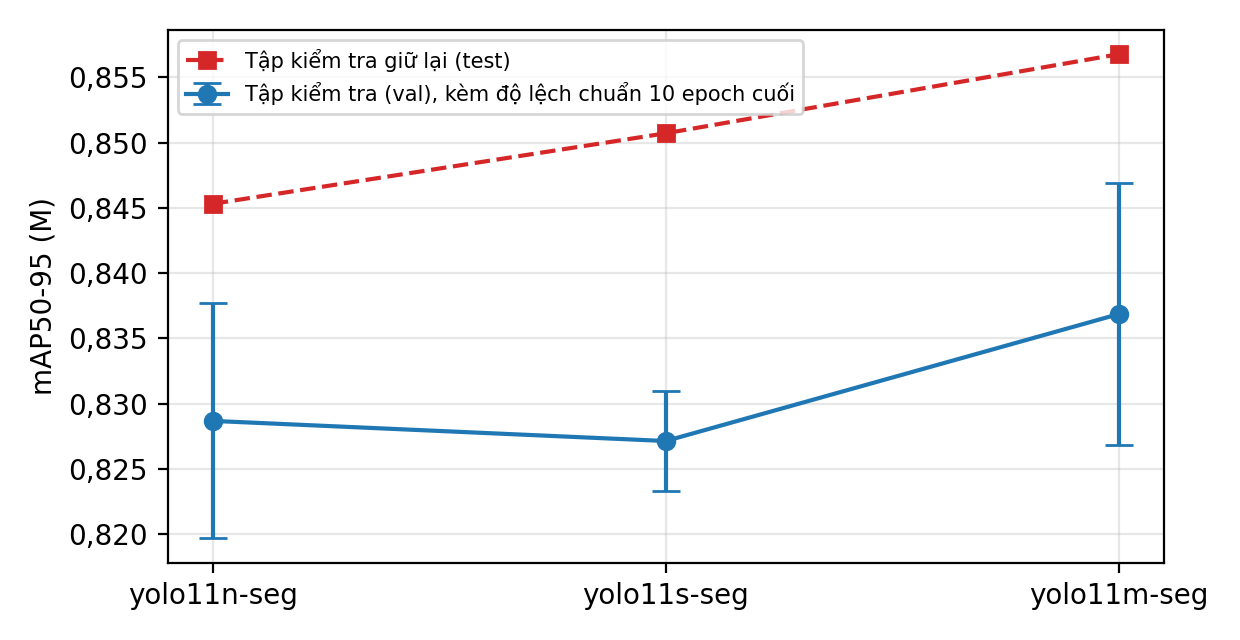
\includegraphics[width=0.64\textwidth]{val_vs_test.png}
\caption{mAP50-95 mặt nạ của ba mô hình trên hai tập đánh giá. Thanh sai số là độ lệch chuẩn của
chính mô hình đó trong mười epoch cuối. Các thanh sai số phủ lên nhau, và hai đường không cùng
hình dạng --- dấu hiệu cho thấy nên đọc bảng xếp hạng này một cách dè dặt.}
\label{fig:gap}
\end{figure}

So với bài phát hiện đối tượng ở bài tập trước, tình hình ở đây có nhỉnh hơn một chút: ở đó thứ tự
ba mô hình đảo hẳn khi đổi tập đánh giá, còn ở đây mô hình lớn nhất giữ được vị trí đầu ở cả hai
tập. Em cho rằng khác biệt này có lý do: phân đoạn đòi hỏi định vị chính xác tới từng điểm ảnh, nên
sức biểu diễn thêm của mô hình lớn có chỗ để phát huy, trong khi ở bài phát hiện với bốn lớp dễ
phân biệt thì nó không có việc gì để làm. Dù vậy, bằng chứng vẫn mỏng, và kết luận thận trọng là:
nếu ứng dụng cần viền thật sát thì chọn mô hình lớn hơn có cơ sở; nếu chỉ cần khoanh vùng ở mức
thông thường thì yolo11n-seg đã đủ, với \nparams{} triệu tham số so với \mparams{} triệu.

\textbf{Về thời gian huấn luyện}, mô hình m chỉ chậm hơn mô hình n \timeratio{} lần (\mminutes{}
phút so với \nminutes{} phút) dù nặng gấp \paramratio{} lần về tham số. Tỉ lệ này không phản ánh
chi phí tính toán thật: với bộ dữ liệu cỡ này trên GPU T4, phần lớn thời gian mỗi epoch dành cho
việc đọc và tăng cường ảnh chứ không phải cho phép nhân ma trận. Muốn so sánh chi phí của ba mô
hình thì phải đo thời gian suy luận trên cùng một lô ảnh.

\section{Hạn chế}

\textbf{Tập test nhỏ.} Phần giữ lại chỉ có \ntest{} ảnh và \ntestobj{} vùng mặt nạ. Với cỡ mẫu đó,
chênh lệch vài phần nghìn điểm mAP hoàn toàn có thể đổi chiều chỉ vì vài ảnh khó rơi vào hay không
rơi vào tập. Đây là lý do báo cáo đối chiếu thêm với tập val thay vì chỉ đọc một cột số.

\textbf{Số epoch còn ngắn.} Ba mô hình đạt mAP val cao nhất ở epoch \nbestepoch{}, \sbestepoch{} và
\mbestepoch{}, tức đường cong đã gần phẳng nhưng cơ chế dừng sớm với \patience{} epoch kiên nhẫn
chưa hề kích hoạt. Nếu chạy dài hơn, mô hình lớn --- vốn đang chậm chân hơn trong mất mát huấn
luyện --- có thể còn tiến thêm.

\textbf{Mỗi cấu hình chỉ chạy một lần.} Em ước lượng nhiễu bằng dao động giữa các epoch ở cuối quá
trình huấn luyện; đây là cách xấp xỉ. Cách chặt chẽ là chạy lại mỗi mô hình với vài hạt giống ngẫu
nhiên rồi so sánh phân bố, như kiểu kiểm định theo cặp em dùng ở hai bài tập đầu.

\textbf{Bài toán một lớp.} Chọn bộ dữ liệu một lớp làm phần phân tích lỗi nghèo đi: không có nhầm
lẫn giữa các lớp để mà bàn. Nếu làm lại, em sẽ cân nhắc \texttt{carparts-seg} với 23 lớp để ma trận
nhầm lẫn nói được nhiều hơn, chấp nhận thời gian huấn luyện dài hơn.

\section{Kết luận}

Em đã huấn luyện ba cỡ mô hình YOLO11 cho bài phân đoạn đối tượng trên bộ \dataname{} theo đúng một
giao thức, bằng học chuyển giao từ trọng số COCO, và chấm điểm trên phần dữ liệu giữ lại. Kết quả
cao nhất là mAP50-95 mặt nạ \besttestmap{} của \besttest{}, với mAP50 của cả ba mô hình đều trên
0,95.

Hai điều em rút ra. Thứ nhất, chênh lệch giữa chỉ số của mặt nạ và của hộp --- trung bình
\maskboxgap{} điểm --- cho thấy phần khó của bài toán nằm ở đường viền, không nằm ở việc tìm ra
vật. Thứ hai, ba cỡ mô hình chênh nhau \paramratio{} lần về tham số nhưng chỉ chênh \testspread{}
điểm mAP, xấp xỉ bằng mức dao động giữa các epoch của chính chúng, và hai chỉ số mAP50 với mAP50-95
còn xếp hạng chúng theo hai thứ tự ngược nhau. Vì vậy báo cáo không khẳng định một mô hình tốt hơn
mô hình khác, mà kết luận rằng câu trả lời phụ thuộc vào việc ứng dụng coi trọng viền sát hay ít
báo nhầm --- và rằng một bảng so sánh chỉ đáng tin khi khoảng cách giữa các dòng lớn hơn nhiễu của
phép đo.

\begin{thebibliography}{9}

\bibitem{he2017}
K. He, G. Gkioxari, P. Dollár, and R. Girshick,
``Mask R-CNN,''
in \emph{Proc. IEEE Int. Conf. Computer Vision (ICCV)}, 2017, pp. 2961--2969.

\bibitem{bolya2019}
D. Bolya, C. Zhou, F. Xiao, and Y. J. Lee,
``YOLACT: Real-Time Instance Segmentation,''
in \emph{Proc. IEEE/CVF Int. Conf. Computer Vision (ICCV)}, 2019, pp. 9157--9166.

\bibitem{khanam2024}
R. Khanam and M. Hussain,
``YOLOv11: An Overview of the Key Architectural Enhancements,''
arXiv preprint arXiv:2410.17725, 2024.

\bibitem{bochkovskiy2020}
A. Bochkovskiy, C.-Y. Wang, and H.-Y. M. Liao,
``YOLOv4: Optimal Speed and Accuracy of Object Detection,''
arXiv preprint arXiv:2004.10934, 2020.

\bibitem{lin2014}
T.-Y. Lin \emph{et al.},
``Microsoft COCO: Common Objects in Context,''
in \emph{Proc. European Conf. Computer Vision (ECCV)}, 2014, pp. 740--755.

\bibitem{yosinski2014}
J. Yosinski, J. Clune, Y. Bengio, and H. Lipson,
``How transferable are features in deep neural networks?''
in \emph{Advances in Neural Information Processing Systems (NeurIPS)}, vol. 27, 2014, pp. 3320--3328.

\bibitem{li2020}
X. Li \emph{et al.},
``Generalized Focal Loss: Learning Qualified and Distributed Bounding Boxes for Dense Object
Detection,''
in \emph{Advances in Neural Information Processing Systems (NeurIPS)}, vol. 33, 2020, pp.
21002--21012.

\bibitem{everingham2010}
M. Everingham, L. Van Gool, C. K. I. Williams, J. Winn, and A. Zisserman,
``The PASCAL Visual Object Classes (VOC) Challenge,''
\emph{International Journal of Computer Vision}, vol. 88, no. 2, pp. 303--338, 2010.

\bibitem{jocher2023}
G. Jocher, J. Qiu, and A. Chaurasia,
``Ultralytics YOLO,'' phần mềm mã nguồn mở, 2023. [Trực tuyến]. Có tại:
\url{https://github.com/ultralytics/ultralytics}

\end{thebibliography}

\end{document}
